\documentclass[14pt,a4paper, oneside]{extreport}
\usepackage{amsmath}
\XeTeXinputencoding "utf8"
\usepackage{fontspec}

\defaultfontfeatures{Mapping=tex-text}
\newfontfamily{\cyrillicfont}{Linux Libertine O}

\usepackage{unicode-math}
\setmathfont[math-style=ISO]{Asana Math}

\usepackage{polyglossia}
\setdefaultlanguage{russian}
\setotherlanguage{english}

%--------------------------------------------------------------

\makeatletter%%%%% <---- Литература с точкой а не скобки
\bibliographystyle{unsrt}
\renewcommand{\@biblabel}[1]{#1.} 
\makeatother

\usepackage{array,delarray}
\usepackage{multirow}
\usepackage{rotating}
\usepackage{graphicx}
\usepackage{graphics}
\usepackage{float}
\usepackage{lscape}
\usepackage{setspace}
\usepackage{color}

%%%%%%%%%%%%%%%%%%%%%%%%%%%%%%%%%%%%%%%%%%%%%%%%%%%%%%%%%%
\renewcommand \labelitemi{\bfseries --}




\begin{document}


\pagestyle{fancy}

\thispagestyle{empty}

\renewcommand{\headrulewidth}{0pt}
\begin{center}
\small Федеральное государственное бюджетное образовательное 

учреждение высшего образования \vspace{2ex}

 
<<РОССИЙСКАЯ АКАДЕМИЯ НАРОДНОГО ХОЗЯЙСТВА 

И ГОСУДАРСТВЕННОЙ СЛУЖБЫ 

ПРИ ПРЕЗИДЕНТЕ РОССИЙСКОЙ
ФЕДЕРАЦИИ>>

\vspace{2ex}

\bfseries
ЭКОНОМИЧЕСКИЙ ФАКУЛЬТЕТ

НАПРАВЛЕНИЕ 38.04.01 ЭКОНОМИКА

МАГИСТЕРСКАЯ ПРОГРАММ <<ЭКОНОМИКА И ФИНАНСЫ>>
\end{center}

\vfill


\noindent\small Группа ЭиФ-2016
\hfill
\parbox[t]{20em}{\centering\small
Кафедра <<Макроэкономики>>

\mbox{ }

\textbf{Допустить к защите}

заведующий кафедрой

\mbox{ }

\rule{8em}{0.5pt} Н.Л. Шагас

\mbox{ }

<<\rule{2em}{0.5pt}>> \rule{5em}{0.5pt} 201\rule{1em}{0.5pt} г. }

\mbox{ }

\mbox{ }

\begin{center}\bfseries
МАГИСТЕРСКАЯ ДИССЕРТАЦИЯ

\mbox{ }

\large
ТЕМА МАГИСТЕРСКОЙ ДИССЕРТАЦИИ 

ПРОДОЛЖЕНИЕ ТЕМЫ МАГИСТЕРСКОЙ ДИССЕРТАЦИИ 

\end{center}

\vfill

\noindent\normalsize
студент-магистрант

\noindent
Иванов Иван Иванович 
\hfill /\rule{6em}{0.5pt}/\rule{6em}{0.5pt}/

\hfill\makebox[13em]{\hfill\footnotesize (подпись) \hfill\hfill (дата) \hfill}

\noindent
научный руководитель


\noindent
к.э.н., доцент Сидоров Сидор Сидорович 
\hfill /\rule{6em}{0.5pt}/\rule{6em}{0.5pt}/

\hfill\makebox[13em]{\hfill\footnotesize (подпись) \hfill\hfill (дата) \hfill}



%\noindent
%консультант
%
%\noindent
%д.э.н., профессор Петров Петр Петрович
%\hfill /\rule{6em}{0.5pt}/\rule{6em}{0.5pt}/
%
%\hfill\makebox[13em]{\hfill\footnotesize (подпись) \hfill\hfill (дата) \hfill}



\vfill\vfill

\begin{center}
\normalsize Москва\\ 2016г.
\end{center}
\normalsize

%%%%%%%%%%%%%%%%%%% ОГЛАВЛЕНИЕ %%%%%%%%%%%%%%%%%%%%%%%%%%%%%%%%%%%%%%
\newpage

\thispagestyle{fancy}

\tableofcontents


      


\chapter*{Введение}

%Включение введения в соодержание
\addcontentsline{toc}{chapter}{Введение}

Для осуществления монетарной политики Центральный Банк может использовать не только традиционные инструменты, но и словесные интервенции (open mouth operations). Суть словесных интервенций очень хорошо иллюстрирует история, которая произошла в США в 1970-1980 гг., в эпоху, которая вошла в мировую историю как Великая инфляция. 

В 1958 г. была опубликована статья экономиста Филиппса, в которой он обнаружил достаточно четкую отрицательную связь между инфляцией и безработицей в Англии за прошедшие 70 лет. Проверка этой работы на американских данных подтвердила взаимосвязь. Кривую Филиппса стали интерпретировать как некую возможность выбора между высокой инфляцией и высокой безработицей~\cite{phillips1958relation}.

Любому политику безработица кажется более значимой социальной проблемой, нежели инфляция и он хочет ее победить любыми доступными средствами. Самым популярным средством по борьбе с безработицей является экспансионистская монетарная политика, состоящая в расширении денежной массы. Именно это и было сделано президентом США Ричардом Никсоном в начале 1970-х гг. в ходе погони за низкой безработицей и высокой инфляцией.

К сожалению, план Никсона удался только наполовину, он добился высокой инфляции, но сбить безработицу не смог, а кривая Филиппса в этот период перестала существовать. 

Все западные страны так или иначе поэкспериментировали с кривой Филиппса и в итоге обрекли 1980-е гг. на обуздание высокой инфляции.

В 1979 г. главой ФРС становится Пол Волкер, который принимает решение очень жестко бороться с инфляцией, однако экономические агенты не верят в заявления ФРС и продолжают ожидать высоких темпов инфляции. Пол Волкер увеличивает процентные ставки и отправляет экономику в краткосрочную рецессию, тем самым сбивая ожидания и уменьшая инфляцию в течение своего председательства с 11,22\% до 3,66\%. 

Таким образом, Пол Волкер заслужил репутацию принципиального борца с высокой инфляцией. Общество верило в его обещания, и при каком-либо макроэкономическом шоке ему достаточно было просто подать сигнал о намерении что-то сделать, и общество сразу же перестраивало свои ожидания в соответствии с этим сигналом.

Таким образом ФРС, заработав устойчивую репутацию, оставляла неизменной величину традиционных инструментов, однако целевые переменные изменялись именно в том направлении, которое требовалось ФРС.

Будем подразумевать под информационными интервенциями сигналы, которые подает Центральный банк для того, чтобы достичь определенного уровня целевой переменной при неизменных величинах традиционных инструментов.

На первый взгляд, речь о возможности регулирования экономики посредством информационных интервенций кажется полным абсурдом, однако существуют центральные банки, которые успешно применяют этот инструмент на практике. Примером такого центрального банка является Резервный Банк Новой Зеландии~(РБНЗ)~\cite{guthrie2000open}.

Целью данной работы является проверка гипотезы влияния словесных интервенций Банка России на динамику валютного курса и процентной ставки. Для достижения цели были поставлены задачи: 

\begin{enumerate}
\item провести критический обзор теоретических работ для выявления механизма воздействия словесных интервенций на динамику макроэкономических переменных;

\item провести критический анализ эмпирических подходов, применяемых для исследования влияния словесных интервенций на динамику различных макроэкономических переменных;

\item собрать и предварительно обработать статистические данные, необходимые для проведения собственных расчетов;

\item построить и оценить модели для проверки влияния словесных интервенции на динамику ставки процента и валютного курса;

\item сформулировать выводы о работоспособности словесных интервенций как инструмента монетарной политики в России.
\end{enumerate}

В первой главе работы будут рассмотрены теоретические работы, освещающие механизмы влияния центральных банков на макроэкономику посредством сигналов.

Во второй главе будут рассмотрены эмпирические работы. После изучения существующих в научной среде подходов к оценке эффективности словесных интервенций как инструмента монетарной политики будет сделан выбор в пользу одного из подходов для проверки работоспособности интервенций на российских данных. 

В третьей главе будут поставлены гипотезы для исследования, осуществлен сбор данных и проведена проверка поставленных гипотез. В заключении будут приведены основные итоги исследования.

%%% Возвращаем нормальную нумерацию глав! 

\titleformat{\chapter} 
    {\normalfont\bfseries\large}
    {\thechapter}{1 em}{\normalfont\bfseries}
    
    
\chapter{Теоретические исследования влияния словесных интервенций на динамику макроэкономических переменных}

\section{Будущее монетарной политики: центральный банк как армия \\ сигнальщиков}

В 1999 году в июле в Оксфорде проходила конференция «Социальные науки и будущее», на которой выступил Бенджамин Фридман\footnote{This paper was initially prepared for the conference on «Social Science and the Future» held at Oxford, U.K., July 7-8, 1999.}. 

Фридман говорил об угрозах и вызовах, которые коснутся монетарной политики в течение первой четверти нового века. Он поднял на обозрение достаточно большое количество проблем, с которыми  центральные банки будут вынуждены столкнуться, и поставил под сомнение возможность проведения монетарной политики в том виде, в котором она присутствует в макроэкономике сегодня. 
 
 Фридман отметил, что публичные заявления различных ЦБ и другие более тонкие сигналы с их стороны приводят к немедленным изменениям цен и доходностей на финансовых рынках, которые в свою очередь приводят к изменению других экономических переменных: 
 
«Сегодня, действительно, широко распространено мнение, которое заключается в том, что центральные банки ровным счетом ничего не должны делать. После достаточно четкого заявления ЦБ о своих намерениях, рынок сделает всю работу~за~него»~\cite{friedman1999future}.

Фридман отмечает, что если на секунду представить себе масштабы экономики и масштабы деятельности какого бы то ни было центрального банка, то можно очень сильно удивиться. 

Например, cтоимость валового продукта США составляет около 17 триллионов долларов за 2015 год. При этом вся банковская сфера, включая ФРС вносит в эту стоимость около 100 миллиардов долларов. Если ФРС изменит величину резервов на 2\%, то многие сочтут такой жест за жесткую монетарную политику, однако, по сути, вклад в экономику страны при таком изменении со стороны ФРС будет ничтожен. 

Сам факт того, что какой бы то ни было центральный банк может влиять на экономику просто-напросто поражает воображение, и возникает устойчивое ощущение, что покупка или продажа любым ЦБ ценных бумаг вообще не играет для экономики никакой роли. Тем не менее никто не сомневается в том, что если завтра будет увеличена ставка процента, то в краткосрочном периоде это приведет к спаду в производстве, а в долгосрочном победит инфляцию. 

Одним из стандартных объяснений такой способности влиять на такие большие рынки такими малыми операциями является то, что операции ЦБ в корне отличаются от операций, осуществляемых другими участниками рынка.

При покупке ценных бумаг ЦБ увеличивает резервный счет банка-продавца, тем самым увеличивая общий объем резервов в экономике и наоборот. ЦБ является единственным участником рынка, способным увеличивать или уменьшать величину резервов. Тот факт, что любой коммерческий банк должен иметь какой-то резерв, делает ЦБ в некотором роде монополистом по созданию этих резервов. 

Вся монетарная политика сфокусирована на существовании различных взаимоотношений между финансовым  и нефинансовым экономическими мирами. Домашние хозяйства и фирмы ищут банки, которые могли бы предоставить им кредиты. Банки могут сделать это только в том случае, если ЦБ создает деньги. При этом ЦБ как поставщик резервов играет в этом процессе решающую роль. Когда ЦБ сокращает предложение резервов, коммерческие банки сокращают кредитование, и процентная ставка фиксируется на более высоком уровне. 

Можно рассмотреть сценарий, когда у центрального банка есть возможность сыграть на ожиданиях экономических агентов, просигнализировав о своих намерениях и изменив краткосрочные ставки, никак не изменяя величину инструмента.  

Однако эта логика имеет смысл только в том случае, если Центральный банк обладает среди агентов определенным авторитетом и действительно может повлиять на краткосрочные процентные ставки, когда придет время. Эта способность, в свою очередь, опирается на роль Центрального банка как монопольного поставщика резервов. 

Стоит отметить, что в наши дни в сфере денежного предложения происходит ряд институциональных изменений. 
В последние годы широко распространились новые технологии, которые позволяют урегулировать сделки в альтернативной обычным деньгам форме. 

Различные электронные платежные системы привели к тому, что спрос на наличные денежные остатки среди экономических агентов снизился. Спрос банков на резервы остался устойчивым, но также снизился. 

Будущее туманно, однако вполне возможен вариант развития событий, который приведет к тому, что может появиться самостоятельная платежная система, которой люди доверяют и в формировании которой ЦБ не будет принимать никакого участия.

Многие коммерческие лица, у которых нет никакой банковской лицензии осуществляют выпуск различного рода «смарт-карт», с помощью которых можно оплачивать покупки. При существовании достаточно высокого уровня доверия к подобной системе люди смогут расплачиваться друг с другом посредством таких карт.  

Сегодня уже практически все платежи в развитых экономиках осуществляются безналично. Новая система расчетов  по-прежнему включает использование банковских денег, но только в качестве начального основания. 

Однако существует еще более безрадостная для центральных банков перспектива. В ближайшем будущем вполне может появиться глобальная платежная система, в которой расчет между сторонами сделок происходит без участия третьей стороны --- гаранта. Сегодня достаточно значительные шаги в этом направлении сделал «биткойн», но до глобальной общепризнанной платежной системы этой криптовалюте предстоит добираться через огромное количество барьеров.

Так в 2014 году Банк Англии\footnote{ Банк Англии о биткойнах: http://www.businessinsider.in/Everyone-Is-Baffled-By-Alan-Greenspans-Comment-About-Bitcoin/articleshow/26873628.cms} и министерство финансов Российской федерации\footnote{Министерство финансов РФ о биткойнах: http://www.vedomosti.ru/finance/articles/2014/10/06/realnyj-shtraf-za-virtualnye-dengi} высказали свои опасения, что при росте популярности системы «Биткойн»  можно потерять контроль над инфляцией.  Кроме того  правительства различных стран отмечают что «Биткойны» активно используются на теневых рынках. Также многие эксперты, в том числе экс-глава ФРС США Алан Гринспен, считают что «Биткойн» демонстрирует многие признаки спекулятивного пузыря\footnote{Алан Гринспен о биткойнах: http://www.businessinsider.in/Everyone-Is-Baffled-By-Alan-Greenspans-Comment-About-Bitcoin/articleshow/26873628.cms}.

Тем не менее присутствует очень высокая угроза монополии ЦБ, состоящая в децентрализации мировой денежной системы, к которой в ближайшем будущем ЦБ придется как-то приспосабливаться.

Одним из направлений активной деятельности ЦБ в данном направлении является сотрудничество с правительством. Вместе они образуют достаточно большой государственный сектор экономики. Правительство может осуществлять выплаты и требовать уплаты налогов в тех формах, которые выгодны ЦБ для поддержания своей монополии. Однако при выполнении основных рыночных принципов, таких как свободная конкуренция и хорошо развитые институты, государственный сектор будет занимать незначительную долю экономики, и при дальнейшем росте безналичных расчетов в частном секторе ЦБ будет терять контроль над денежной базой. 


\section{Словесные интервенции Центрального Банка}
Вслед за Фридманом многие авторы начали активно изучать область информационных сигналов. В таких работах авторы, используя теоретико-игровой подход для описания взаимодействия центрального банка и общества пришли к выводу, что заявления, выпущенные ЦБ, и выступления их глав в парламентах оказывают существенное влияние на рыночные процентные ставки, стоимости активов и валютный курс. 

Этот отклик происходит в следствие того, что ЦБ предоставляет в ходе таких выступлений важную информацию о своих ближайших политических предпочтениях и перспективах экономики. 

Многие исследователи отмечают, что любое решение, принимаемое центральным банком, преследующим свои цели, должно носить максимально прозрачный характер.

Прозрачность работы центрального банка может быть определена как отсутствие асимметричной информации между монетарными органами и другими экономическими агентами.  Прозрачность его деятельности уменьшает неопределенность. Кроме того, она может повлиять на стимулы разработчиков политики, пытающихся манипулировать мнением частного сектора посредством словесных интервенций и построения репутации.  Все склонны полагать, что повышение прозрачности улучшает экономические показатели.

Тем не менее менее существует мнение, что оптимальным уровнем прозрачности работы центрального банка является некоторый промежуточный уровень. Как это ни парадоксально, высокий уровень прозрачности деятельности ЦБ может привести к неопределенности.  Слишком большой объем информации приводит к перегрузке и путанице~\cite{morris2005central}.

Выделяется несколько различных каналов связи центрального банка и общества~\cite{kohn2003central}:

\begin{enumerate}
\item Пресс-релизы центрального банка. Обычно такие релизы сопровождают какие-либо действия центрального банка или совещания.  Обычно политика таких релизов различается от одного центрального банка к другому и меняется с течением времени.

\item Выступления председателя центрального банка перед парламентом. Председатель ЦБ часто выступает перед парламентам на различные темы. В основном, он сосредотачивается на разъяснении конгрессменам текущей экономической ситуации и экономических перспектив.


\item Речи председателя центрального банка и другие публичные выступления. Обычно глава монетарного ведомства говорит на огромное количество тем перед совершенно разными аудиториями. Тематика таких выступлений очень сильно различается. 

\item Публикация целевых ориентиров и прогнозов для ряда макроэкономических переменных, раскрытие макроэкономических моделей и своих оценок текущего состояния экономики.
\end{enumerate}



\section{Информационный канал}

Осуществление монетарной политики происходит через чёрный ящик монетарной политики: каналы монетарной трансмиссии.

К традиционным каналам монетарной трансмиссии относят процентный и валютный. Кроме того существую банковские каналы, значимость которых ввиду развития финансовых рынков и борьбой с рыночными несовершенствами падает. В последнее время в развитых странах, где процентный канал постепенно перестает функционировать, возрастает роль информационного канала монетарной трансмиссии.

На практике одни из самых важных сдвигов в монетарной политике происходят за счет изменения ожиданий экономических агентов. В связи с тем, что при изменении какого-либо монетарного инструмента, в первую очередь, на него следует отклик ожиданий, управление ими стало важнейшим инструментом монетарного регулирования по всему миру~\cite{boivin2010has}.

Грэми Гатри и Джулиан Райт на примере Резервного Банка Новой Зеландии показали, как именно работает информационный канал в таких ситуациях на примере процентных ставок, и предложили для Новой Зеландии модель монетарной политики, базирующуюся на угрозах~\cite{guthrie2000open}.

Предполагается, что временная структура процентных ставок имеет вид:

\begin{equation}
\frac{1}{T} \sum_{k=0}^{T-1} E_t[R_{t+k,t+k+1}] =  R_{t,t+T},
\end{equation} где $R_{t,t+1}$ --- однодневная ставка процента в день $t$.

Предполагается, что центральный банк для выполнения своих задач имеет предпочтительный уровень процентной ставки на конкретный день, $R_{t,t+T}$. Под таким уровнем подразумевается такая ставка, которой ЦБ смог бы достичь в течение дня с помощью операций на открытом рынке. 

Также предполагается, что ЦБ обладает достаточной репутацией для достижения такой же ставки за счет угрозы применить операции на открытом рынке. 

Это будет происходить благодаря следующему механизму. Предположим, что рыночная ставка овернайт в день $t$ отклонилась от целевого уровня. Тогда центральный банк, используя операции на открытом рынке в $t+1$ день, 
приведет ставку к уровню $R^*_{t+1,t+2} = 2R_{t,t+2} - \hat R_{t,t+1}$. Инвестор, зная, что такое произойдет не будет в день $t$ использовать ставку ниже, чем $\hat R_{t,t+1}$, так как он сможет получить более высокую доходность от двухдневной ставки. Кроме того, никто не будет использовать ставку выше, чем $\hat R_{t,t+1}$, так как зная, что во втором периоде ставка упадет, малая ставка будет означать короткую позицию. Наличие «угрозы» со стороны регулятора подавляет возможность возникновения арбитража.  

Авторы строят свою модель для РБНЗ, который использует операции на открытом рынке для того, чтобы поддерживать величину номинальных денежных запасов на целевом уровне. 

Долгосрочное равновесие ставок поддерживается именно за счет поддержания этого уровня. При фиксации ставки на более высоком уровне из-за словесной интервенции деньги в экономике становятся дороже, денежная база автоматически сокращается, и происходит отклонение от целевого уровня номинальных денежных запасов.

Если экономические агенты не знают предпочтительной ставки банка, частный сектор может вывести её на неправильный уровень. Это отклонение, обозначенное ниже как  $\zeta_s$, с точки зрения центрального банка является нежелательным. Производя словесную интервенцию, центральный банк может обеспечить фиксацию ставки частным сектором на правильном уровне. 

Когда центральный банк посылает словесную интервенцию, он подвергается риску быть неуслышанным и лишиться части своей репутации. Поэтому каждый раз, делая заявление, ЦБ подвергается некоторым издержкам и в конечном счете минимизирует функцию потерь вида

\begin{equation}
\E \left[ \sum_{s=0}^{\infty} e^{-ks} \zeta_s^2 + PV(announcement costs) \right],
\end{equation} где  $PV(announcment costs)$ --- эти самые издержки, $k$ --- ставка дисконтирования для будущих издержек отклонения ставки.

Таким образом, центральный банк, прежде чем допустить заявление, будет ждать критического уровня отклонения ставки от целевого значения. При этом каждый анонс ЦБ приводит к дискретному скачку уровня процентных ставок в желательном направлении. Стоит отметить, что анонсы должны быть непредсказуемыми, иначе частный сектор может предвидеть их и включить информацию о них в процентные ставки.

\section{Теоретико-игровой подход в моделировании словесных интервенций}

Большая часть теоретических моделей, описывающих различные словесные интервенции, реализуют теоретико-игровой подход. В играх такого рода взаимодействуют центральный банк и общество. Общество формирует ожидания, а центральный банк --- величину целевой переменной.

Этот подход был заложен в 1977 г. Кинландом и Прескотом, предложившими динамическую элегантную модель взаимодействия ЦБ и всей остальной экономики~\cite{kydland1977rules}. 

\subsection{Модель Кинланда и Прескота}

Уровень инфляции в экономике напрямую связано с предложением денег. Центробанк вынужден искать золотую середину между уменьшением безработицы и экономическим ростом, к которым может привести увеличение предложения денег, и  издержками от инфляции. Эта взаимосвязь задается кривой Филиппса:

\begin{equation}\label{T3-1}
y = \bar y + b(\pi-\pi^e),
\end{equation}
где $y$ --- ВВП, $\pi$ --- инфляция, $\pi^e$ --- ожидаемый уровень инфляции, $\bar y$ --- потенциальный ВВП.
 
Пусть ВВП и инфляция определяются в результате следующей игры. На первом этапе этой игры общество формирует свои инфляционные ожидания. На втором этапе ЦБ определяет уровень инфляции и предложение денег в экономике. 
Функция полезности ЦБ представляет собой функцию социальных потерь вида:

\begin{equation}\label{T3-2}
U_b = -(y - y^0)^2 - \alpha (\pi - \pi^0)^2.
\end{equation}
Полезность общества зависит от того, насколько точным оказался его прогноз инфляции:

\begin{equation}\label{T3-3}
U_p = -(\pi - \pi^e)^2.
\end{equation}

Найдем равновесие в этой игре при нулевом целевом уровне инфляции. Сначала решим задачу ЦБ при данной ожидаемой инфляции:

\begin{equation}\label{T3-4}
U_b = - (\bar y + b(\pi - \pi^e) - y^0)^2 - \alpha \pi^2 \to \max_\pi.
\end{equation}

Получаем стратегию ЦБ вида:

\begin{equation}\label{T3-5}
\pi(\pi^e)=\frac{b}{b^2+\alpha} (y^0- \bar y + b \pi^e).
\end{equation}

Максимизируя $U_p$ по ожидаемой инфляции, при условии  $\pi=\pi(\pi^e)$, мы получим, что в равновесии 

\begin{equation}\label{T3-6}
\pi^e = \pi = \frac{b}{\alpha} (y^0 - \bar y) \mbox{ и } y = \bar y.
\end{equation}

Последний результат получен, исходя из предположения о наличии рациональных ожиданий у общества: уровень инфляции, который установится в результате монетарной политики, проводимой ЦБ, не может отличаться от ожидаемого (здесь исключаются возможные случайные колебания). Общество предвидит действия ЦБ и корректирует ожидания. 

Полученное равновесие не является оптимальным по Парето. Действительно, такого же объема выпуска $\bar y$ можно было бы достигнуть и при $\pi=\pi^0$. Однако этот уровень инфляции несостоятелен во времени. Например, предположим, что ЦБ обещает $\pi=\pi^0$, и общество формирует свои ожидания на таком уровне. Тогда у ЦБ будет стимул обмануть эти ожидания, т.к. $\pi(\pi^0)>\pi^0$. При предположении, что не существует никаких факторов, которые заставили бы ЦБ сдержать свое слово касательно уровня инфляции, уровень инфляции $\pi=\pi^0$ не может быть достигнут.

Сдержать ЦБ от такого оппортунистического поведения могут определенные правила, регулирующие его работу. Чем выше вес инфляции в целевой функции, тем ниже инфляция будет в равновесии. Именно из-за этого в Германии, где была сильна память о гиперинфляции 1922-1923 гг. на протяжении второй половины 20 века инфляция находилась на низком уровне.

Согласно Барро и Гордону, центральный банк может придерживаться целевого показателя инфляции, если между ним и обществом существует определенный уровень доверия. Если изначально банк располагает доверием общества, которое думает, что в ближайшем будущем он не станет печатать деньги, тем самым преследуя инфляционную политику, то банку может быть невыгодно обманывать ожидания общества, так как это повлечет за собой рост инфляционных~ожиданий~и потерю доверия~\cite{barro1981positive}. 

Это можно описать в виде бесконечно повторяющейся игры. Предположим, что в моменты времени $ t=1,2…$  два игрока – банк и общество – играют в следующую игру. Изначально общество ожидает, что банк будет придерживаться политики низкой инфляции: $\pi^e=0$. Банк в каждый момент времени выбирает, какой уровень инфляции – низкий $\pi_L=\pi^0=0$ или высокий $\pi_H=\pi(0)=\frac{b}{b^2+\alpha} (y^0 - \bar y)$  следует реализовывать. Если банк обманывает ожидания общества и реализует высокий уровень, то начиная со следующего момента времени, общество ожидает уровень инфляции, соответствующий равновесию в рассмотренной выше динамической модели: $\pi^e=\frac{b}{\alpha} (y^0- \bar y)$.

Пусть $\delta$ --- фактор дисконтирования для ЦБ. Сравним дисконтированную полезность банка когда он всегда придерживается политики низкой инфляции и когда он  отклоняется от неё в момент времени $t=1$. В первом случае дисконтированный выигрыш ЦБ составит:

\begin{equation}\label{T3-7}
W_{b1} =  -\frac{1}{1-\delta}(y^0-\bar y)^2,
\end{equation}.
во втором:
\begin{equation}\label{T3-8}
W_{b2} =  -(y^0-\bar y)^2 \frac{\alpha}{b^2+\alpha}-\frac{c}{1-\delta}(y^0 - \bar y)^2(1+\frac{b^2}{\alpha}).
\end{equation}

Равновесие с низкой инфляцией возможно, если $W_{b1}>W_{b2}$ или $\delta \ge \frac{\alpha}{2\alpha+b^2}$.

При прочих равных ЦБ будет придерживаться политики низкой инфляции при достаточно высоком $b$ или при достаточно малом $\alpha$, так как в таких случаях равновесная инфляция будет слишком мала.

Таким образом, при определенных предпосылках относительно функций общества и центрального банка в совершенном в подыграх равновесии уровень инфляции будет высоким. Для эффективной борьбы с шоками предложения и ожидаемой инфляцией необходимо, чтобы у центрального банка был выработан мощный репутационный механизм.

\subsection{Репутация центрального банка}

Для того чтобы ЦБ смог успешно осуществлять словесные интервенции, экономические агенты, условно говоря, должны видеть в Центральном банке «угрозу», которая в любой момент может вмешаться в экономику. Для того чтобы быть «угрозой» Центральный банк, безусловно, должен обладать монополией на резервы, однако этого недостаточно. Кроме всего прочего Центральному банку необходима репутация, заработать которую очень сложно. Именно репутационные механизмы задействовал в 1980-х гг. Пол Волкер.

Если ЦБ обладает репутацией беспринципного борца с высокой инфляцией, то общество, доверяя его обещаниям, закладывает в зарплаты низкие инфляционные ожидания. Обманув общество, центральный банк добьется высокого ВВП на какое-то время, но при этом потеряет свою репутацию. 

Теоретико-игровая модель, описывающая репутационные механизмы центрального банка, была предложена Барро~в~1986~г.~\cite{barro1986reputation}.

Пусть взаимодействие ЦБ и общества происходит на протяжении двух периодов. В каждый момент времени $t = \{1,2\}$ общество формирует инфляционные ожидания $\pi_t^e$, после ЦБ определяет уровень инфляции $\pi_t$. ВВП в момент времени $t$ задается
кривой Филлипса:
\begin{equation}
y_t = \bar{y} +b(\pi_t-\pi_t^e). 
\end{equation}
В игре существует три игрока: общество в момент времени $t = 1$, общество в момент времени
$t = 2$ и центральный банк. Выигрыш общества в момент времени $t$ равен
\begin{equation}
U_{pt}=-(\pi_t^e-\pi_t)^2.
\end{equation}
Центральный банк может относиться к одной из двух разновидностей. Первая разновидность — оппортунист, имеющий функцию полезности
\begin{equation}
U_b = y_1 - \bar y - \frac{a}{2} (\pi_1 - \pi_0)^2 + \beta (y_2 - \bar y - \frac{a}{2} (\pi_2 - \pi_0)^2),
\end{equation}
 где $\pi_0=0$ --— оптимальный уровень инфляции, $\beta <1$ --- фактор дисконта. Вторая разновидность ЦБ — принципиальный борец с инфляцией, устанавливающий
$\pi_1=\pi_2=0$ независимо от того, какими являются инфляционные ожидания общества. Пусть $p$ ---
вероятность того, что центральный банк окажется оппортунистом.

Если центральный банк является беспринципным борцом с инфляцией, то его поведение не
определяется внутри модели. Нас интересует, как поведет себя банк-оппортунист. Будем решать игру методом обратной индукции и рассмотрим
сначала поведение оппортуниста в момент времени $t = 2$. Запишем целевую функцию ЦБ
как
\begin{equation} 
U_b = b (\pi_1 - \pi_1^e) - \frac{a}{2} \pi_1^2 + \beta (b(\pi_2 - \pi_2^e) - \frac{a}{2} \pi_2^2). 
\end{equation}

Максимизируя ее по $\pi_2$, получаем
\begin{equation} 
\pi_2^* = \frac{b}{a}.
\end{equation}
Найдем теперь $\pi_2^e$. Пусть $\lambda$ --- вера общества относительно того, что центральный банк имеет тип $1$ после момента времени $t=1$. Математическое ожидание выигрыша общества в момент $t=2$ будет равно
\begin{equation}
E(U_{p^2}) = -(1-\lambda)\pi_2^e - \lambda (\pi_2^e - \frac{b}{a})^2. 
\end{equation}

Соответственно, уровень ожидаемой инфляции, максимизирующий $E(U_p^2)$, будет равен 

\begin{equation}
\pi^e_2(\lambda) = \lambda \frac{b}{a}.
\end{equation}

Найдем $\lambda$. Если $\pi_1 \ne 0$, то $\lambda=0$ (так как принципиальный ЦБ предпочитает нулевую инфляцию). Логично, что для ЦБ второго типа любая стратегия, предполагающая $\pi_1 \notin \{0,\frac{b}{a}\}$, будет доминироваться стратегией, в которой $\pi_1 = \frac{b}{a}.$ Следовательно, у ЦБ второго типа $\pi_1$ может принимать только два значения: $0$ и $\frac{b}{a}$. Пусть ЦБ второго типа играет стратегию, предполагающую выбор $\pi_1 = 0$ с вероятностью $q$. Веру общества при этом можно найти по формуле Байеса. 

\begin{equation}
\lambda = \frac{p q}{1-p+qp}, 
\end{equation}
где $qp$ --- вероятность того, что ЦБ относится к первому типу и выбирает нулевую инфляцию, $1-p$ --- вероятность того, что ЦБ относится ко второму типу (что автоматически означает $\pi_1=0$). 

Найдем выигрыш ЦБ, если в момент $t=1$ он играет стратегию $\pi_1 = 0$. Мы получим

\begin{equation}
W_0(q) = -b \pi_1^e + \beta \left(b \left(\frac{b}{a}-\lambda \frac{b}{a} \right) - \frac{a}{2} \left(\frac{b}{a} \right)^2 \right) = \beta \frac{b^2}{a} \left(\frac{1}{2} - \frac{p q}{1-p+qp} \right)-b \pi_1^e.
\end{equation}

Если в момент $t=1$ ЦБ выбирает $\pi_1 = \frac{b}{a}$, то он выигрывает величину равную 

\begin{equation}
W_1(q) = W_1 = \left(b \left(\frac{b}{a}-\pi_1^e \right) - \frac{a}{2} \left(\frac{b}{a} \right)^2 \right) - \beta \frac{a}{2} \left(\frac{b}{a}\right)^2 = \frac{b^2}{2a} (1-\beta) - b \pi_1^e.
\end{equation}

Заметим, что $W_0(q)$ убывает по своему аргументу $q$, а $W_1$ не зависит от $q$. Всего возможно три равновесия:

\begin{enumerate}
\item равновесие, в котором $q=0$, то есть $\pi_1 = 0$. Это осуществимо при $W_0(1) \ge W_1$, или $\beta \le \frac{1}{2}$;

\item равновесие, в котором $q=1$, то есть $\pi_1 = \frac{b}{a}$. Это осуществимо при $W_0(0) \le W_1$, или $\beta \ge \frac{1}{2(1-p)}$;

\item равновесие, в котором $q \in (0,1)$, то есть центробанк играет смешанную стратегию. Вероятность $q$ является решением уравнения $W_0(q) = W_1$ или $q= \frac{1-p}{p} (2 \beta -1)$. Такое равновесие осуществимо при $\frac{1}{2} < \beta < \frac{1}{2(1-p)}.$

\end{enumerate}

Таким образом, низкая инфляция сегодня означает низкие инфляционные ожидания на завтрашний день. Низкоинфляционное равновесие в модели возможно при достаточно высоком $\beta$, то есть если ЦБ оценивает выгоды в будущем выше, чем выгоды в настоящем. 

\subsection{Объявление ЦБ целевых ориентиров} 
Одним из вопросов, обсуждаемых в теоретико-игровой литературе, связанной с моделированием словесных интервенций, является вопрос важности объявления центральным банком своих намерений, выражающихся в фиксировании целевых уровней для ключевых макроэкономических переменных.   
  
Стэфан Палмквист в своей работе отмечает, что тенденцией последнего времени является активный переход различных стран к режиму таргетирования инфляции. Целью своей работы он ставит разработку модели, которая помогла бы понять как центральный банк может оказывать на экономику влияние за счет объявления своих целей или намерений. Конструируя свою модель на основе работ Кинланда и Прескота, Барро и Гордона, автор пытается объяснить, почему центральные банки иногда объявляют свои цели и намерения частному сектору, а иногда~нет~\cite{palmqvist1998central}.

Конструируемая модель предполагает следующую последовательность действий:

\begin{itemize}
\item центральный банк объявляет о том, что в течение следующего периода будет проводиться политика таргетирования инфляции;

\item экономические агенты формируют свои инфляционные ожидания;

\item после формирования ожиданий происходит  шок предложения;

\item центральный банк реализует свою политику;

\item таргетируемый уровень инфляции становится понятным для частного сектора.
\end{itemize}

В статье предполагается наличие информационной асимметрии следующего характера: ЦБ знает текущие цели монетарной политики, а частный сектор нет.

Поведение частного сектора описывается с помощью кривой предложения 

\begin{equation}
y_t = \a (\pi_t - \pi_t^e) + \e_t,
\end{equation} где $y_t$ --- логарифм ВВП, $\pi_t$ --- текущая инфляция, $\pi^e_t$ --- инфляционные ожидания частного сектора, $\e_t$ --- независимые шоки с нулевым математическим ожиданием и одинаковой дисперсией, $\a >0 $ --- влияние неожиданной инфляции на текущий выпуск. Предполагается, что ожидания экономических агентов рациональные. В контексте модели величина $\a$ понимается как сигнал частному сектору о характере политики, которую проводит центральный банк. 

Центральный банк в ходе осуществления своей политики стремится выбрать инфляцию таким образом, чтобы минимизировать ожидаемую функцию потерь. 

\begin{equation}
V_t = \E_{t_1} \left[ \sum_{j=t}^{\infty} \beta^{j-t} L_j \right ],
\end{equation} где $\beta \in (0,1)$ --- фактор дисконтирования, а $L_j$ --- функция потерь ЦБ в период $t$, которая имеет вид

\begin{equation}
L_t = \frac{1}{2} \left[ (\pi_t - \pi_t^{CB})^2 + \lambda (y_t-y^*)^2 \right] +S(\a),
\end{equation} где $y^*>0$ --- оптимальный уровень выпуска, $\lambda >0$ --- вес, характеризующий предпочтения ЦБ относительно проводимой политики, $\pi^{CB}$ --- таргетируемый уровень инфляции, $S(\a)$ --- потери от сигнала $\a$. 

Предполагается, что таргетируеый уровень инфляции может принимать два значения: низкое и высокое. 

Функция издержек от сигналинга, $S(\a)$ предполагется линейной. В случае, если ЦБ объявляет цель по инфляции, то он обеспечивает себе дополнительные издержки $f$. 

\begin{equation}
S(\a) = f + \a, \a >0
\end{equation}

Далее автор в своей модели ищет равновесие в такой игре. Автор приходит к выводу, что при разных ограничениях на параметры в такой игре может существовать два типа равновесных стратегий: никогда не заниматься сигналингом и сигналить, если текущая цель по инфляции является низкой, не сигналить, если текущая цель по инфляции является высокой. То есть слабые центральные банки никогда не будут делать заявления, в то время как сильные будут. 

\subsection{Неоднозначность прозрачности деятельности ЦБ}

Сегодня любой центральный банк должен нести ответственность за свои решения и соответствовать самым высоким стандартам порядочности и компетентности. Любое решение, принимаемое независимым центральным банком, преследующем свои непосредственные цели, должно носить максимально прозрачный характер. Мало кто ставит под сомнение то, что в таком широком смысле ЦБ должен быть прозрачным. Однако в научной литературе ведутся активные дебаты, связанные с прозрачностью деятельности ЦБ в узком смысле. 

Тем не менее, вопрос о том, должен ли ЦБ публиковать свои прогнозы, объявлять численную цель по инфляции для осуществления максимально эффективной монетарной политики, является достаточно спорным.

Многие ведущие экономисты, занимающиеся вопросами монетарной политики, сегодня видят основной её задачей управление ожиданиями населения~\cite{svensson2000should},~\cite{woodford2005central}.

Управление ожиданиями населения ставит в центр внимания политику ЦБ, связанную с осуществлением коммуникаций. Многие ЦБ отнеслись с энтузиазмом к данной идее и приняли явный режим инфляционного таргетирования. Тем не менее достаточно малое внимание уделялось последствиям прозрачности ЦБ для информативности цен.

Цены для экономики являются не только пропорцией обмена одного товара на другой, но и имеют второстепенную роль --- роль передачи информации об основах экономики и разных шоках~\cite{hayek1945use}.

 Для того, чтобы знать как управлять чужими ожиданиями, ЦБ должен получить от экономики некоторые сигналы, которые сами являются продуктом ожиданий. Для того, чтобы направить экономику в правильное русло, ЦБ необходима хорошая информация о её текущем состоянии. Если сигналы, получаемые им, будут неинформативны, то возникнет проблема управления. Таким образом, с одной стороны, ЦБ вынужден учиться на ожиданиях рынка, с другой, управлять ими. Для того чтобы эффективно манипулировать экономическими событиями, ЦБ должен быть бдительным наблюдателем этих самых событий. 
 
Вся дилемма при этом заключается в том, что чем больше ЦБ раскрывает информации, тем менее точные сигналы он получает от экономики, информационная ценность сигналов ухудшается. 
 
В условиях неопределенности доступ к новой информации позволяет агенту, получившему его, принимать решения, которые лучше подходят для конкретных обстоятельств. При выявлении частной информации другими агентами, её наличие отражается на результатах, показываемых рынком.

Наличие общедоступной информации в какой-то степени приводит к уменьшению значения частной информации участников рынка.

Общедоступная информация включает в себя информацию о глубинных основах экономики. Она координирует экономических агентов. При этом общие сигналы, не имеющие глубинных основ, в той же самой степени играют координирующую роль. 

Агенты при вере в то, что информация, получаемая о ЦБ, имеет глубинную основу о функционировании
экономики, уделяют меньше внимания своей частной информации и собственным независимым оценкам. Происходит вытеснение частного мнения, и рынок перестает функционировать как агрегатор разнообразной частной информации о мире. Возникает некоторая информационная экстерналия. 

С одной стороны, улучшенная способность ЦБ читать информацию обеспечивает агентам информацию повышенного качества и приводит к росту авторитетности его мнения. С другой стороны, на рынке происходит координация ожиданий, и канал, через который несогласные агенты могли бы выразить своё мнение, заглушается. Чистый эффект увеличения прозрачности ЦБ является достаточно неоднозначным. 

Одной из часто рассматриваемых в научной литературе моделей, связанной с прозрачностью деятельности ЦБ, является модель Morris и Shin, построенная в теоретико-игровом ключе~\cite{morris2005central}.

Главный вывод из этой модели состоит в том, что центральный банк не должен делать всю информацию, которой он располагает, общедоступной. 

Однако эта статья была воспринята в штыки и встречена достаточно суровой критикой со стороны многих видных экономистов. 

Таким образом, из теоретического обзора можно заключить, что многие теоретические модели, основанные на теоретико-игровом подходе, подталкивают исследователей к выводу, что сильные, обладающие репутацией ЦБ могут эффективно использовать словесные интервенции для достижения своих целей.

Управление ожиданиями стало важнейшим инструментом монетарного регулирования по всему миру. Многие ЦБ стали успешно использовать сигналы для достижения своих целей. Во второй главе будут рассмотрены работы, посвященные изучению применения словесных интервенций на практике.


\chapter{Эмпирические исследования влияния словесных интервенций на экономику}

В этой главе будут рассмотрены эмпирические работы, посвященные исследованию функционирования информационного канала и применению словесных интервенций как инструмента монетарной политики. 

Тема словесных интервенций в монетарной политике является относительно новой. Однако несмотря на её новизну, к сегодняшнему дню сформировалось огромное количество различных подходов к работе со словесными интервенциями.

Как уже было отмечено, впервые о словесных интервенциях заговорили совсем недавно. В 1989 г. Кук и Хан опубликовали работу, в которой исследовали реакцию рынка на изменение ставок по федеральным фондам. Они обнаружили, что в период с 13 сентября 1974 г. по 5 октября 1979 г. ставки по казначейским ценным бумагам сроком от трех месяцев до двадцати лет значительно отреагировали на изменение целевых ставок по федеральным фондам, опубликованным в Wall Street Journal. Нормы по трех, шести и двенадцати месячным облигациям подскочили примерно на 50 базисных пунктов в ответ на публикацию об изменении целевого уровня по долгосрочным ценным бумагам на один процентный пункт. Авторы интерпретировали это как свидетельство того, что ФРС изменяет процентные ставки посредством словесных интервенций~\cite{cook1989effect}.

Позднее, в 2004 г., Дэниэл Тронтон активно поднимает вопрос о том, нужно ли ФРС проводить операции на открытом рынке для того, чтобы изменять ставки, или же ему достаточно просто заявлять о своих намерениях. В ходе своего исследования автор описывает произошедший в конце 1970-х г. эпизод и внимательно анализирует его~\cite{thornton2004fed}.

Для анализа были использованы ежедневные наблюдения, собранные за 1974 - 1979 гг. Рассматривалось изменение эффективной процентной ставки по федеральным фондам, $\Dt ff$, и изменение в трехмесячной ставке по казначейским векселям,  $\Dt tb_3$.   Изменение в целевой ставке по федеральным фондам рассматривалось в двух формах: объявленное изменение целевого уровня,  $\Dt fftar^{WSJ} $ и фактическое, $\Dt fftar^{A} $. Все целевые уровни, опубликованные в WSJ, были разделены на те, которые совпали с фактическим,  $\Dt fftar_A^{WSJ}$ и на те, которые не совпали с фактическими, $\Dt fftar_{NA}^{WSJ}$. Фактические также были разделены на совпавшие с WSJ, $\Dt fftar_{WSJ}^A$ и не совпавшие, $\Dt ffrar_{NWSJ}^A$.

По причине того, что ставки по казначейским векселям и ставки по федеральным фондам являются коинтегрированными, оценивалась модель коррекции ошибок вида 

\begin{equation}
\Dt x_t = \Psi(L) \Dt x_{t-1} + ECT_{t-1} \dt + \dt fftat_t \beta + \e_t,
\end{equation} где $\Dt x'_t = (\Dt ff_t, \Dt tb3_t)$.

Модель была оценена с использованием изменений, отраженных в WSJ, и фактических изменений. Тест Йохансона показал ранг коинтеграции равный единице для всех оценок. 

Оценка модели показывает, что изменение ставки при несовпадении изменения цели в WSJ и в реальности различаются, однако это различие является статистически незначимым. В конечном счете автор приходит к выводу, что нет никаких оснований полагать, что в рассматриваемый период имели место эффективные словесные интервенции. 

Тем не менее, у многих исследователей есть весомые основания полагать, что в другие временные периоды в других странах имели место эффективные словесные интервенции. Работы этих авторов будут рассмотрены ниже.

Грэми Гатри и Джулиан Райт исследуют в своей статье то, как словесные интервенции могут использоваться как инструмент монетарной политики на примере Новой Зеландии. В своей работе они приходят к выводу, что словесные интервенции приводят к изменению ставок в течение всего рассматриваемого периода~\cite{guthrie2000open}.

Всего авторами было рассмотрено 2149 дневных наблюдений. Все выходные и праздники были выброшены из рассмотрения. Все ставки были измерены на 11 часов утра. 

Для словесных интервенции были построены специальные дамми-переменные. Для их конструирования были использованы статьи из Reuters, в которых содержались слова «Reserve Bank», «Monetary» и «Donald Brash» (руководитель Резервного Банка Новой Зеландии (РБНЗ), который делал в этот период много заявлений).

Также был использован поиск по основным фамилиям чиновников в Гугле. Таким образом, были идентифицированы еще несколько заявлений, не рассмотренных ранее. Вся хронология событий была перепроверена по основным публикациям РБНЗ. После сбора были удалены все статьи, которые не содержали информацию о каких-то монетарных ограничениях или сопровождались изменением величины инструмента.

Все наблюдения, которым соответствовали какие-то заявления центрального банка, были выделены дамми-переменной $STATEMENT = 1$. Все заявления ЦБ были структурированы с помощью дополнительных дамми.

$TIGHTEN=1$ --- если заявление РБНЗ подразумевает ужесточение монетарной политики;

$TIGHTEN=-1$ ---  если заявление РБНЗ подразумевает смягчение монетарной политики;

$SURPRISE = 1$ ---  если заявление является сюрпризом, а не формальным релизом информации. Все официальные заявления, которые должны были быть реализованы в заранее объявленные сроки были закодированы $SURPRISE = -1$. Если это заявление прозвучало в какой-то официальной речи, которая была заранее анонсирована, то $SURPRISE = 0$. 

Эмпирическая работа велась вокруг сюрпризных заявлений. Дамми-переменная $A$ формировалась следующим образом:

\begin{equation}
A = \begin{cases}
1,&\text{если } STATEMENT=1 \wedge TIGHTEN=1 \wedge SURPRISE =1;\\
-1,&\text{если }  STATEMENT=1 \wedge TIGHTEN=-1 \wedge SURPRISE =1;\\
0,&\text{иначе.}
\end{cases}
\end{equation}

Переменная А используется как стандарная мера словесных интервенций. Значение $А=1$ означает заявление об ужесточении. Значение  $А= -1$ означает заявление о смягчении.  

Далее авторы решали две задачи. Прямую --- как заявления центрального банка влияют на экономические переменные, и двойственную к ней --- можно ли по изменению какой-то экономической переменной предсказать характер заявления Центрального Банка. Начнем с описания двойственной задачи.

 Для того чтобы предсказать характер заявления ЦБ мы должны оценить порядковую пробит-модель следующего вида:

\begin{equation}
A_t = \begin{cases} -1 &\text{, если } b(L) \Delta X_{t-1} + c(L) A_{t-1} + \varepsilon_t < \gamma_1, \\
\mbox{ }0 &\text{, если } \gamma_1 < b(L) \Delta X_{t-1} + c(L) A_{t-1} + \varepsilon_t < \gamma_2, \\
\mbox{ }1 &\text{, если } \gamma_2 < b(L) \Delta X_{t-1} + c(L) A_{t-1} + \varepsilon_t, 
\end{cases}
\end{equation} где $X_{t}$ --- различные виды ставок или обменный курс, $\varepsilon_t \sim iid N (0, \sigma^2)$, $b(L) = \sum_{j=0}^m b_j L^j$, $c(L) = \sum_{j=0}^n c_j L^j$. 

Модель оценивалась методом максимального правдоподобия. С помощью теста Вальда проверялись гипотезы о незначимости отдельных коэффициентов. Оптимальная величина $m$ и $n$ выбиралась с помощью критерия Шварца. Были использованы различные показатели $X_t$. Во всех оцениваемых моделях критерий Шварца показал, что лагов быть не должно. То есть запаздывание переменной не помогает в выявлении характера заявления ЦБ. Значимым первое запаздываение оказалось только для случая валютного курса. 

Однако при увеличении на 25 базисных пунктов валютного курса изменение в вероятности того, что будет сделано заявление, у авторов получилось ничтожным. Исходя из этого факта при решении прямой задачи авторы предполагают, что изменения в прошлом периоде рассматриваемых переменных не оказывают влияния на заявление РБНЗ.

Для решения прямой задачи, задачи влияния словесных интервенций на динамику валютного курса и процентных ставок была построена VAR модель, в которой все заявления рассматривались как экзогенные переменные.

У РБНЗ в рассматриваемый период имелась цель монетарной политики. Он использовал операции на открытом рынке для того, чтобы таргетировать постоянный номинальный запас денежных средств. РБНЗ учитывал отклонение от этой цели внутри постоянного прогнозируемого уровня в номинальных единицах. 

Модель, рассматриваемая в работе, имела вид: 

\begin{equation}\label{VAR}
\left\{
\begin{aligned}
\Delta X_t = \alpha + \alpha_x (L) \Delta X_{t-1} + \alpha_{FE}(L) FE_t + \alpha_A(L) A_t + \alpha_D \bar D_t + u_{1t}, \\
FE_t = \beta + \beta_X(L) \Delta X_{t-1} + \beta_{FE}(L) FE_{t-1} + \beta_A(L) A_t + \beta_D \bar D_t + u_{2t},
\end{aligned} \right.
\end{equation} где $\bar D_t$ --- вектор из дамми переменных для таких дней недели как день до и день после каждого официального выходного, $FE_t$ --- ошибки прогноза расчета движения денежных средств РБНЗ.

Количество лагов в многочленах выбиралось с помощью критерия Шварца из 10 запаздываний.

В модели были сделаны два идентифицирующих предположения:

\begin{enumerate}

\item анонсы РБНЗ не зависят от лагированных или одновременных значений процентных ставок, обменных курсов и ошибок прогноза РБНЗ;

\item ошибки прогноза расчёта денежных средств не зависят от одновременных или лагированных изменений процентных ставок или валютных курсов. 
\end{enumerate}

Таким образом, переменные были упорядочены как $A_t \to  FE_t \to X_t$. При таком упорядочивании были построены функции импульсного отклика для каждой из рассматриваемых ставок и валютного курса. Доверительные интервалы для них были построены методом Монте-Карло.

При сюрпризном заявлении происходит прыжок каждой из рассмотренных ставок в течение следующего дня. Чтобы убедиться, что операции на открытом рынке не несут ответственность за найденные изменения, авторы находят количественные оценки реакции макроэкономической переменной на шоки в этих операциях, соответствующие их дневному изменению, используя уравнение~(\ref{VAR}). 
Оказывается, что через операции на открытом рынке можно объяснить лишь часть динамики процентных ставок. 


Марсель Фатнер в своей работе в 2008 г. изучает то же самое явление на примере США, Германии и Японии. Автор отмечает, что за последнее двадцатилетие произошли фундаментальные изменения режима курсовой политики среди многих стран мира. Так США практически отказались от фактических интервенций на валютных рынках и почти полностью сместились к использованию словесных интервенций. Своей целью автор ставит оценку сдвига этого режима и анализ его эффективности~\cite{fratzscher2008communication}. 

 Автор извлек из службы Reuters все новостные заявления за период с 1990 по 2003 гг. Были взяты дневные данные. Котировки валютных курсов были взяты на момент закрытия торговли на бирже Нью-Йорка. Автор отмечают, что всеобъемлющая доступность новостей этой службы позволяет экономическим агентам узнать о наличии словесной интервенции  практически моментально. В связи с этим, если информационный канал функционирует нормально, то отклик в динамике валютного курса будет получен в тот же день.

Все заявления были классифицированы следующим образом:

\[IO_t = \begin{cases}
1,&\text{ если заявление должно привести к укреплению национальной валюты};\\
-1,&\text{ если заявление должно привести к ослаблению национальной валюты};\\
0,&\text{  если заявление носит неоднозначный характер.}
\end{cases}
\]

Классификация при этом делается на основе содержания высказываний. Все сообщения, произошедшие на день, соответствующий совещанию ЦБ относительно изменений в монетарной политике, индексируются нулями. 

Модель, используемая автором работы, формулируется следующим образом:

\begin{equation}
\Dt S_t^{USD/EUR} = \a + \sum_j (\beta^j IA_t^j + \gamma^j IO_t^j) + \dt(i^{US}_t - i^{EA}_t) + \sum_d W_t^d + \e_t,
\end{equation} где $\Dt S_t$ --- изменение в логарифме валютного курса,  $IA_t$ ---валютные интервенции, $IO_t$ --- словесные интервенции,  $W_t$ --- дамми-переменная, отвечающая за день недели, $j \in \{EA, US\}$. Аналогичная модель оценивалась для Японской йены. До 1999 г. для случая Германии рассматривается марка.

При этом волатильность валютного курса моделируется как $EGARCH(1,1)$. Модель оценивалась методом максимального правдоподобия.

С помощью LR - теста автор убеждается в том, что все параметры вносят в модель значимый вклад.  В случае пары евро/доллар при прочих равных интервенция приводит к изменению в курсе в среднем на 0.2\%, в паре доллар/евро (выступление идёт в США) в среднем на 0.12\%, в паре доллар/йена в среднем на 0.15\%.

Автор называет словесную интервенцию эффективной, если она перемещает величину валютного курса в тот же день, когда происходит заявление, в необходимом направлении. Он называет политику успешной, если  в долгосрочной перспективе валютный курс достигает конечной цели.  Политика может быть эффективной, но неуспешной, если валютный курс стабилизируется не на том уровне. Однако эффект успешности вмешательства оценить затруднительно, так как мы изначально не знаем цель этого вмешательства, а также каким образом развивались бы события без него. 

Основным выводом из работы является то, что связь между словесными интервенциями и динамикой валютного курса действительно является эффективным инструментом монетарной политики. Кроме того отмечается, что меры особенно эффективны, когда они идут вразрез с существующей политической мантрой. Стоит отметить, что в таком контексте эффективность словесных интервенций не гарантирует политикам успешного достижения долгосрочных целей по валютной политике. 

Майкл Эрман и Марсель Фатнер в своей работе в 2007 г. рассатривают период с мая 1999 г. по декабрь 2003 г. для ФРС, период с мая 1997 г. по декабрь 2003 г. для Банка Англии и период с января 1999 г. для ЕЦБ~\cite{ehrmann2007communication}.

В качестве источника данных была использована новостная лента Reuters. Было выделено два типа заявлений: о монетарной политике и об экономических перспективах. По аналогии со своими коллегами авторы построили дамми переенные $C_t^{EC}$ и $C_t^{MP}$, принимающие значения 1, 0 и -1. 

Классификацией заявлений при этом занималось два эксперта. Все спорные ситуации в классификации обсуждались отдельно.

Для анализа в статье используется месячная ставка EONIA своп для зоны Евро и месячная ставка LIBOR для США и Великобритании.

Рассматривается модель вида
\begin{equation}
r_t = \a + \lambda r_{t-1} + \beta^{EC} C_t^{EC} + \beta^{MP} C_t^{MP} + \dt X_t + \e_t,
\end{equation} где $r_t$ --- ставка процента, $X_t$ --- вектор контрольных переменных.  Он включает в себя эффекты отдельных дней недели, $\e_t = \sqrt{h_t} \times \nu_t$, $\nu_t \sim iid (0,\sigma_{\nu})$. Компонента $h_t$ описывалась моделью EGARCH(1,1).

При оценивании модели был получен значимый вклад словесных интервенций в изменение ставок.
Далее  базовое уравнение модели было модифицировано. Все заявления разбились на группы с помощью дамми переменной $D_t$, которая принимала значение равное 1, если заявление делало лицо, являющееся главой какого-нибудь комитета, и значение 0, если лицо, делающее заявление, являлось каким-то иным членом комитета. Оценивалось уравнение:

\begin{multline}
r_t = \a + \lambda r_{t-1} + \beta_1^{EC} C_t^{EC} D_t + \beta_2^{EC} C_t^{EC} (1-D_t) + \beta_1^{MP} C_t^{MP} D_t + \\ + \beta_1^{MP} C_t^{MP} (1-D_t) + \dt X_t + \e_t.
\end{multline}


Было получено, что заявления Гринспена и других глав вносят гораздо больший вклад в изменение ставок.  


Синдзи Такаги и Хироки Окада в своей работе в 2013 г. рассматривают словесные интервенции в Японии. В работе исследуется сигнальный эффект интервенций на валютном рынке~
 \cite{takagi2013central}. 

Авторы отмечают что эффективность словесных интервенций зависит от того, является ли центральный банк независимым. Рассматривается месячные данные с 1980 по 2004 гг. Эффективность вмешательства тестируется на промежутке до и после апреля 1998 г., когда независимость центрального банка Японии была закреплена в новом законе. 

Оценивается пробит модель вида:

\begin{equation}
x_t = \a_0 +\a_1 IND_t + \a_2 SEL_t + \a_3 QE_t + u_t, 
\end{equation}где $x$ --- бинарная переменная, которая принимает значение 1, когда направление интервенций согласуется с изменением в монетарной политике и  0, когда нет, $IND$ --- фиктивная переменная для независимости центрального банка, принимающая до апреля 1998 г. значение 1, $SEL$ --- фиктивная переменная для валютных интервенций, $QE$ --- фиктивная переменная для политики количественного смягчения, принимающая значение 1 после марта 2001 г. 

Бинарная переменная $x$ определяется по отношению к целевому ориентиру Банка Японии, используемому на соответствующий период.

В ходе исследования было установлено, что после  становления Банка Японии независимым  сонаправленность интервенций и будущей монетарной политики в Японии ослабла. 


Стоит отметить, что эмпирические методы исследования словесных интервенций достаточно разнообразны. Так, например, Леонардо Мелоси из Лондонской школы экономики в своей работе в 2013 г. разработал DSGE модель, в которой рассмотрел политику сигналов ЦБ на примере ставок~\cite{melosi2013signaling}.
 
Автор оценивал модель методом максимального правдоподобия на данных по США. Было установлено, что сигнальные эффекты монетарной политики являются эмпирически важными и оказывают смягчающее воздействие на инфляцию. Также было установлено, что в условиях шоков спроса сигналы повышают способность ФРС стабилизировать экономику. В случае технологических шоков роль сигналов в стабилизации очень мала. 


Пол Мизен в свой статья от 2009 г. исследовал влияние заявлений президента ЕЦБ на изменение процентных ставок~\cite{mizen2009can}.

В своей работе автор использует непараметрический тест, разработанный Песарном и Тиммерманом (nonparametric test of predictive failure and independence) для проверки влияния словесных интервенций ЕЦБ на динамику процентной ставки. Прежде этот тест в подобном контексте в литературе не использовался~\cite{pesaran2000recursive}. \label{P_T}

Целью тестирования было понять может ли информация, содержащаяся в переменном дискретном индикаторе (заявления председателя ЕЦБ) дать хорошую прогностическую способность к направлению изменения процентной ставки. 

Все переменные были закодированы по шкале от -2 до 2. Для заявлений главы ЕЦБ 0 представляет собой нейтральные заявления или их отсутствие. Значение +2 показывает на заявление, содержащее сильное давление к повышению ставок.
Значение +1 указывает на более мягкое давление. Значения -1 и -2 показывают эквивалентное давление к понижению. В случае ставки её увеличение и снижение также было переведено в шкалу от -2 до 2 (рост менее чем на 0.25 раз эквивалентен +1). Все используемые данные были взяты из работы 
Стефан Герлах~\cite{gerlach2007interest}.

Тест Песарана-Тиммермана предназначен для проверки гипотезы $H_0:$ «Один ряд из дискретных переменных не несет информации об изменчивости другого ряда из дискретных переменных».

Предполагается, что  переменные $y_t$ и $x_t$ принимают $m$  разных дискретных значений. Запишем все наблюдения в виде таблицы размера $m \times m$, где на месте $(i,j)$ стоит количество сопряженных элементов. Пусть $n_{ij}$ --- элементы этой матрицы, $n_{i0}$ ---   сумма элементов в $i$-ой строке, $n_{0j}$ --- сумма элементов в $j$-ой колонке, $n$ --- общая сумма всех наблюдений. 

Следующая статистика при верности гипотезы $H_0$ будет иметь асимптотически нормальное распределение с нулевым математическим ожиданием и некоторой дисперсией:
\begin{equation} 
\sqrt{n} S_n = \sqrt{n} \sum_{i=1}^m [n_{ii}/n-(n_{i0}/n)(n_{0i}/n)].
\end{equation}

Эта статистика может использоваться для проверки нулевой гипотезы. Однако удобнее использовать статистику, приведенную ниже:

\begin{equation}
\chi^2 = \sum_{i,j}^M \frac{[n_{ij}-(n_{i0}n_{oj}/n)]}{(n_{i0}n_{0j}/n)} \sim \chi^2_{(m-1)^2}.
\end{equation}

Статистика  асимптотически имеет распределение Хи-квадрат с $(m-1)^2$ степенями свободы. Гипотеза $H_0$ в данном случае имеет вид $(n_{ii}/n) = (n_{i0}/n)(n_{0j}/n) \qquad \forall i,j$. 

В результате тестирования было установлено, что гипотеза о том, что заявления ЕЦБ не влияют на динамику ставки, отвергается. 

Дональд Кох и Брайн Сак в своей работе, в 2003 г. исследуют словесные интервенции в США.Авторы пытаются выяснить, имеют ли различные типы взаимодействия (пресс релизы, выступления главы ФРС перед Конгрессом, другие речи главы ФРС) схожее влияние на экономику~\cite{kohn2003central}.

Рассматриваются данные с 3 января 1989 г. по 7 апреля 2003 г. (промежуток времени, когда главой ФРС являлся Алан Гринспен). 

Авторы отмечают, что существует определенная трудность с оценкой характера словесных интервенций ФРС и обращают внимание на волатильность финансовых переменных в те дни, когда ФРС делает какое-то заявление. Основная идея работы заключается в том, что если политические заявления оказывают влияние на финансовые переменные, то волатильность в дни выступлений должна для этих переменных быть выше. 

Сосредоточив своё внимание на волатильности авторы избегают необходимости индексировать словесные интервенции посредством дамми-переменной. 

Часть заявлений при этом сопровождается изменением инструмента. Исходя из этого, в статье допускается изменение финансовой переменной на величину инструмента и на неожиданную величину, определяющую словесные интервенции: 

\begin{equation}
\Dt ff'' = \frac{D}{D-d} \times \Dt ff_1,
\end{equation} где $D$ --- количество дней в месяце, $d$ --- номер дня, когда было сделано заявление, $\Dt ff_1$ --- изменение в ставке по фьючерсам.

Эта мера вычислялась для всех дней, в которые происходили заявления ФРС, и устанавливалась равной нулю для всех остальных дней.  

Рассматриваемые переменные также могут быть подвержены значительному влиянию ряда других факторов, в том числе макроэкономических релизов. Некоторые из таких релизов происходили в те же дни, когда и релизы ФРС. Для того чтобы очистить колебания стоимости фьючерсов от таких релизов, была введена переменная $mac''_i$.  Всем дням, в которые релиза не было, соответствует нулевое значение переменной. 

Рассматривалась модель вида

\begin{equation}
\Dt y_t = \beta_0 + \beta_1 \Dt ff''_t + \sum_{t=2}^{n} \beta_i mac''_i + \eta_t,
\end{equation} где $\Dt y_t$ --- изменение стоимости фьючерса.

Авторы приходят к выводу, что волатильность процентной ставки в дни выступлений действительно оказывается выше.

Хелдэр Ферера и Ивандо Фариаб в своей работе, в 2014 году исследовали словесные интервенции в Бразилии~\cite{de2015brazilian}.

 Рассматривались дневные данные с 16 февраля 2004г. по 30 октября 2009г. Модель специфицировалась следующим образом:

\begin{equation}
F_i = \a_0 + \a_1 COM_t + \a_2 + INF_t + \a_3 GDP_t + \a_5 EX_t + \a_6 BIR_t + \a_7 G40_t + \e_t,
\end{equation} где $F_t$ --- изменение процентной ставки на рынке фьючерсов, $COM_t$ --- словесные интервенции. В качестве контрольных переменных рассматриваются: $INF_t$ --- инфляция, $GDP_t$ --- экономический рост, $EX_t$ --- валютный курс, $BIR_t$ --- базовая процентная ставка, $G40_t$ --- значение индекса, включающего в себя 40 самых ликвидных облигаций.  

Исследование подтвердило, что словесные интервенции ЦБ Бразилии влияют на динамику процентной ставки в необходимом ЦБ направлении.

Отдельно стоит отметить, что в большинстве работ, представленных в данном обзоре и  проверяющих наличие влияния словесных интервенций на динамику различных макроэкономических переменных, все оценки заявлений, сделанных центральными банками, делаются экспертно и, в определенном смысле, носят достаточно субъективный характер.

Обобщенные результаты критического анализа эмпирических работ приведены в таблице~\ref{tab1}.


\begin{longtable}{|m{2.5cm}|m{3.5cm}|m{2.5cm}|m{6cm}|}
	\caption{Критические выводы обзора эмпирических работ}\label{tab1}\\
	\hline
	Авторы & Выборка & Метод & Результат исследования \\ 
	\endfirsthead
	\multicolumn{4}{r}{Окончание таблицы \ref{tab1}}\\\hline
	Авторы & Выборка & Метод & Результат исследования \\ \hline
	\endhead
	\hline
	\endfoot
	\hline
	\endlastfoot
\hline
  		Дэниэл Тронтон, 2004 & США, дневные данные, 1974-1979 гг. & Процедура Йохансона & Влияние словесных интервенции ФРС на динамику ставок отсутствует  \\
  		\hline
  		Грэми Гатри и Джулиан Райт, 1999 & Новая Зеландия, дневные данные, 1 января 1979 г. - 30 сентября 1997 г.& Структурные VAR & Словесные интервенции влияют на динамику ставок и валютного курса  \\ 
  		\hline
  		Марсель Фатнер, 2008 & США, Германия, Япония, дневные данные с 1990 по 2003 гг.  & Метод максимального правдоподобия, EGARCH & Словесные интервенции являются эффективным инструментом монетарной политики по отношению к валютному курсу \\ 
  		\hline
  		Майкл Эрман и Марсель Фатнер, 2007 & США, Великобритания, Евросоюз, дневные данные с 1997 по 2000 гг. & Метод максимального правдоподобия, EGARCH & Словесные интервенции влияют на динамику процентных ставок \\ 
  		\hline
  		Пол Мизен, 2009 & Евросоюз, дневные данные из работы Стефан Герлах & Тест Песарана-Тиммермана & Гипотеза о том, что заявления ЕЦБ не влияют на изменение ставки, отвергается  \\
  		\hline
  		Дональд Кох и Брайн Сак, 2003 & США, дневные данные 1989 - 2003 гг. & Метод наименьших квадратов & Заявления ФРС влияют на динамику цен на фьючерсы  \\
  		\hline
  		Леонардо Мелоси, 2013 & США, квартальные 1970-2006 гг. & DSGE & Сигналы повышают способность ФРС стабилизировать экономику  \\
  		\hline
  		Хелдэр Ферера и Ивандо Фариаб, 2014 & Бразилия, дневные данные 2004-2009 гг. &Метод максимального правдоподобия, EGARCH& Словесные интервенции ЦБ эффективно влияют на динамику процентной ставки \\
  		\hline
\end{longtable}

В целом, обзор эмпирических работ указывает на наличие влияния словесных интервенций на динамику различных макроэкономических переменных в разных  странах. В изученных работах отклик на изменение переменной, отвечающей за словесные интервенции, оказывается значимым. 

В третьей главе рассмотренные выше подходы будут применены для оценки эффективности словесных интервенций Банка России.


\chapter{Оценка эффективности заявлений Банка России}

\section{Формулировка задач для исследования}

В конце 2014 г. Банк России принял решение перейти к режиму инфляционного таргетирования. 

Как отмечает Ксения Юдаева, основной целью центрального банка при инфляционном таргетировании является влияние на инфляцию, переменную, на которую центральный банк не может влиять напрямую. В формировании инфляции важную роль играют ожидания населения, поэтому важнейшую роль для развития Банка России начинает играть информационная политика~\cite{UDAEVA}. 

Банк России постепенно иначе выстраивает свою политическую линию, повышая уровень предсказуемости и прозрачности. Информационная политика центрального банка движется по направлению к международным стандартам. Уже публикуются календарь совещаний Совета директоров Банка России, график публикаций решений об изменении ключевой ставки. Регулярно публикуются «Доклады о денежно-кредитной политике», в которых обосновываются те или иные решения, принятые Банком России. 

С 2016 г. в целях повышения эффективности информационного канала Банк России планирует предпринять следующие меры:

\begin{itemize}
\item публиковать протоколы и сокращенные стенограммы заседаний совета директоров не позднее, чем через месяц после заседания,

\item раскрывать содержание экономико-математических моделей, используемых при принятии решений в области монетарной политики;

\item ежеквартально публиковать целевые ориентиры и сценарные прогнозы основных макроэкономических агрегатов;

\item наладить по примеру большинства центральных банков публикации на сайте Банка России результатов научно-исследовательских работ по монетарной политике и финансовому сектору в форме рабочих документов и дискуссионных документов.
\end{itemize}

Несмотря на постепенное налаживание управления ожиданиями рынка, по мнению Ксении Юдаевой, Банк России пока не имеет репутации банка, способного эффективно использовать информационный канал для достижения своих целей \cite{UDAEVA}. 

Тем не менее после перехода к режиму плавающего валютного курса председатель Банка России Эльвира Набиуллина периодически говорит в своих выступлениях о том, что в ближайшее время произойдет с валютным курсом. 

Такие заявления можно расценивать как словесные интервенции и попытаться посмотреть, реально ли эти интервенции оказывают на валютный курс какое-то влияние.

Интерес представляет решение следующих двух задач:

\begin{enumerate}

\item[\textbf{Прямая задача:}] Оказывают ли в России словесные интервенции влияние на динамику валютного курса и процентных ставок?

\item[\textbf{Двойственная задача:}] Можно ли по динамике валютного курса или процентной ставки предсказать характер словесной интервенции (ужесточающая или смягчающая)?
\end{enumerate}

\section{Данные}

Выборка охватывает период с 1 января 2015 года по 31 декабря 2015 года. Для решения поставленных задач были использованы дневные данные. 

Все данные о динамике обменного валютного курса (рублей за доллар США)  были взяты из базы данных  «Финам». Значения индекса РТС были взяты с сайта Московской Биржи. При расчётах используются цены на момент закрытия биржи. Процентная ставка МИАКР по кредитам сроком на один день и информация о валютных интервенциях были взяты из базы данных Банка России. Цены на нефть марки Brent были взяты из базы данных «Финам».

Для конструирования дамми-переменной, отвечающей за словесные интервенции использовался новостной архив газеты «Ведомости». На языке программирования Python был написан код, который вытащил из архива все статьи, в заголовках которых фигурировали словосочетания: «Набиулл», «Центробанк», «Юдаев», «Банк России», «ЦБ». Для последующей обработки были сохранены текст каждой статьи, её заголовок и ссылка на неё. Код, использованный для выкачки, приведен в приложении А.  

В ходе изучения статей были сформированы следующие дамми-
переменные:

\begin{enumerate}
\item[] $S=1$, если в рассматриваемый день Банком России было сделано заявление, подразумевающее что в будущем будет произведено ужесточение монетарной политики;

\item[] $S=-1$, если в рассматриваемый день Банком России было сделано заявление, подразумевающее что в будущем будет произведено смягчение монетарной политики;

\item[] $S=0$, если в рассматриваемый день не было сделано ни одного заявления или все заявления носили нейтральный характер.
\end{enumerate}

\begin{table}[h]
	\begin{center}
		\caption{Описание переменных}\label{varieble}
		\begin{tabular}{|m{3cm}|m{8cm}|}
  		\hline
  		Переменная & Описание \\ \hline
    	$USD$ & валютный курс (рублей за доллар)  \\ \hline
  		$RTS$ & индекс РТС \\ \hline
  		$MIACR$ & процентная ставка МИАКР по кредитам сроком на один день \\ \hline
  		$VAL$ & объем валютных интервенций\\ \hline
  		$OIL$ & цены на нефть \\ \hline
  		$D$ & переменная, принимающая значение 1, если рассматриваемый день - первый рабочий день после выходных или последний рабочий день перед выходными \\ \hline
  		$S$ & словесные интервенции (-1--- смягчение, 1 --- ужесточение, 0 --- характер интервенции неясен) \\ \hline
		\end{tabular}
	\end{center}
\end{table}

Всеобъемлющая доступность новостной информации позволяет узнать экономическим агентам о наличии словесных интервенций практически моментально. В связи с этим отклик в целевой переменной должен произойти в тот же день, когда произошла словесная интервенция или на следующий день после словесной интервенции.

Будем по аналогии с Марселем Фатшером называть словесную интервенцию эффективной, если она перемещает величину валютного курса, ставки МИАКР или индекса РТС в необходимом направлении в течение одного дня~\cite{fratzscher2008communication}.

\begin{table}[h]
	\begin{center}
		\caption{Проверка гипотезы единичного корня}\label{unitroot}
		\begin{tabular}{|m{2.5cm}|m{6cm}|m{6cm}|}
  		\hline
  		Переменная & P-значение для теста в уровнях & P-значение для теста в первых разностях \\ \hline
    	$USD$ & $0.83$ & $0.00$  \\ \hline
  		$RTS$ & $0.39$ & $0.00$ \\ \hline
  		$MIACR$ & $0.55$ & $0.00$ \\ \hline
  		$OIL$ & $0.84$ & $0.00$ \\ \hline
		\end{tabular}
	\end{center}
\end{table}


Отдельно стоит отметить, что гипотеза о том, что ряды $USD$, $RTS$, $MIACR$ и $OIL$ относятся к классу $I(1)$ не отвергается на 5\% уровне значимости. Исходя из этого во всех дальнейших моделях будут рассматриваться первые разности указанных переменных. Результаты тестирования гипотезы единичного корня для рассматриваемых временных рядов представлены в таблице~\ref{unitroot}.


\section{Решение двойственной задачи}

Проверим можно ли по динамике валютного курса, ставки процента или индекса РТС предсказать характер заявления, которое делает Банк России. Для этого оценим следующую порядковую пробит-модель:

\begin{equation}
S_t = \begin{cases} -1 &\text{ если } b(L) \Delta X_{t-1} + c(L) S_{t-1} + \varepsilon_t < \gamma_1 \\
\mbox{ }0 &\text{ если } \gamma_1 < b(L) \Delta X_{t-1} + c(L) S_{t-1} + \varepsilon_t < \gamma_2 \\
\mbox{ }1 &\text{ если } \gamma_2 < b(L) \Delta X_{t-1} + c(L) S_{t-1} + \varepsilon_t 
\end{cases}, 
\end{equation}

где $X_{t}$ --- ставка МИАКР, обменный курс или индекс РТС, $\varepsilon_t \sim iid N (0, \sigma^2)$, $b(L) = \sum_{j=1}^m b_j L^j$, $c(L) = \sum_{j=1}^n c_j L^j$.

Модель оценивалась методом максимального правдоподобия. Количество лагов $n$ и $m$ выбиралось с помощью минимизации критерия Шварца из десяти запаздываний для каждой переменной. Перебор показал, что оптимальны значения $n=1$ и $m=1$. Код, с помощью которого производился отбор, приведен в приложении Б. После оценивания с помощью статистики Вальда проверялась гипотеза о незначимости регрессии в целом.

В таблице~\ref{stask} представлены результаты решения двойственной задачи. Каждая из рассмотренных порядковых пробит регрессий незначима на 5\% уровне значимости. Аналогичный результат был получен для динамики цен на нефть. 

\begin{table}[H]
	\begin{center}
		\caption{Решение двойственной задачи}\label{stask}
		\begin{tabular}{|m{6cm}|m{4cm}|}
\hline
Объясняющие переменные & P-значение для проверки гипотезы $b_0 = c_0 =0$  \\ \hline
$\Dt USD_{t-1}$, $S_{t-1}$ & 0.1344   \\ \hline
$\Dt RTS_{t-1}$, $S_{t-1}$ & 0.0715   \\ \hline
$\Dt MIACR_{t-1}$, $S_{t-1}$ & 0.3625   \\ \hline
$\Dt OIL_{t-1}$, $S_{t-1}$ & 0.1302   \\ \hline
		\end{tabular}
	\end{center}
\end{table}

Таким образом гипотеза о том, что динамика переменных, рассмотренных выше, не несёт никакой информации о будущих заявлениях Банка России не отвергается.


\section{Решение прямой задачи с помощью методологии VAR}

Проверим влияют ли словесные интервенции Банка России в течение рассматриваемого периода на динамику валютного курса, процентной ставки и индекса РТС. Для исследования данного вопроса будем использовать методологию VAR.

В работе Гатри и Райта, уже упоминавшейся выше, у РБНЗ имелась цель монетарной политики. ЦБ таргетировал постоянный номинальный запас денежных средств. РБНЗ ежедневно публикует на своём сайте свой прогноз по номинальному запасу денежных средств и учитывает его, осуществляя операции на открытом рынке~\cite{guthrie2000open}. 

В течение рассматриваемого периода Банк России придерживается режима таргетирования инфляции. Вполне уместно было бы специфицировать модель похожим образом, используя вместо ошибок прогноза расчета движения денежных средств отклонение текущего уровня инфляции от таргетируемого. Однако в условиях дневных данных это является невозможным в связи со спецификой расчета инфляции. Попробуем специфицировать модель несколькими различными способами отличными от работы Новозеландских коллег и сравним полученные результаты между собой. Код для оценки соответствующих моделей и построения функций импульсного отклика приведен в приложении В.

\textbf{Первая спецификация:}

\begin{equation}
\left\{
\begin{aligned}
\Dt X_t &= \a + \sum_{i=1}^p \a_{xi} \Dt X_{t-i} + \sum_{i=1}^p \a_{si} S_{t-i} +\a_d D_t +  u_{1t}, \\
S_t &= \b + \sum_{i=1}^p \b_{xi} \Dt X_{t-i} + \sum_{i=1}^p \b_{si} S_{t-i} + \b_d D_t +  u_{2t}.
\end{aligned}
\right.
\end{equation}
 
При оценивании модели количество лагов выбиралось из 10 запаздываний с помощью критерия Шварца. Он показал, что оптимальным является взять одно запаздывание. 

При решении двойственной задачи было получено, что заявления Банка России не зависят от лагированных или одновременных значений процентной ставки МИАКР, валютного курса и индеса РТС. Исходя из этого факта упорядочим переменные как $S_t \to \Dt X_t$.

Функции импульсного отклика валютного курса, индекса РТС и ставки МИАКР на заявление Банка России при такой спецификации и идентифицирующих предположениях будут иметь вид, представленный на рис.~\ref{otkl_1}. Функции импульсного отклика представлены с 95\% доверительными интервалами, построенными с помощью бутстрапа.

\begin{figure}[h]
\begin{minipage}[H]{0.49\linewidth}
\center{\footnotesize{Валютный курс} \\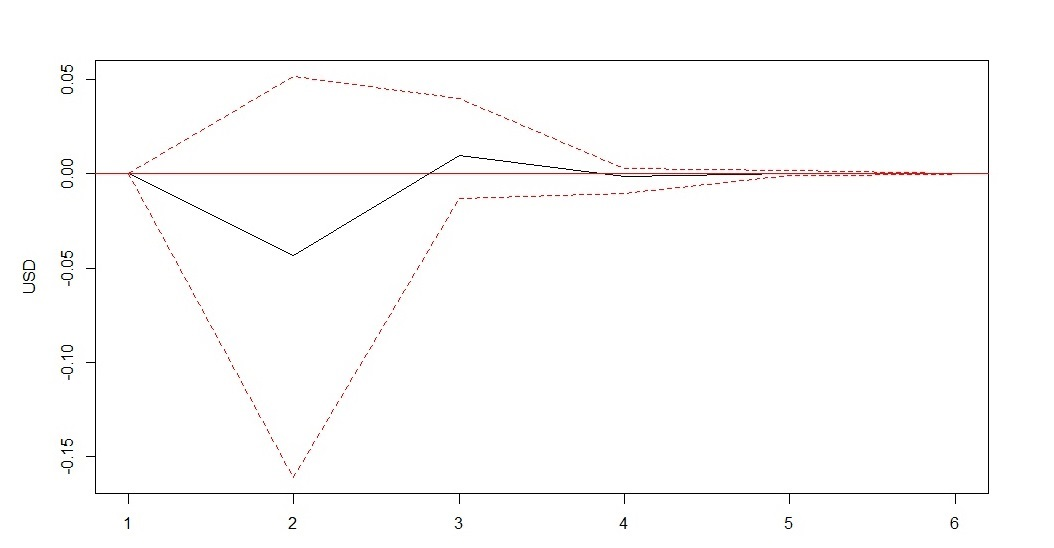
\includegraphics[width=1\linewidth]{1_usd_res}}
\end{minipage}
\hfill
\begin{minipage}[H]{0.49\linewidth}
\center{\footnotesize{Индекс РТС} \\ 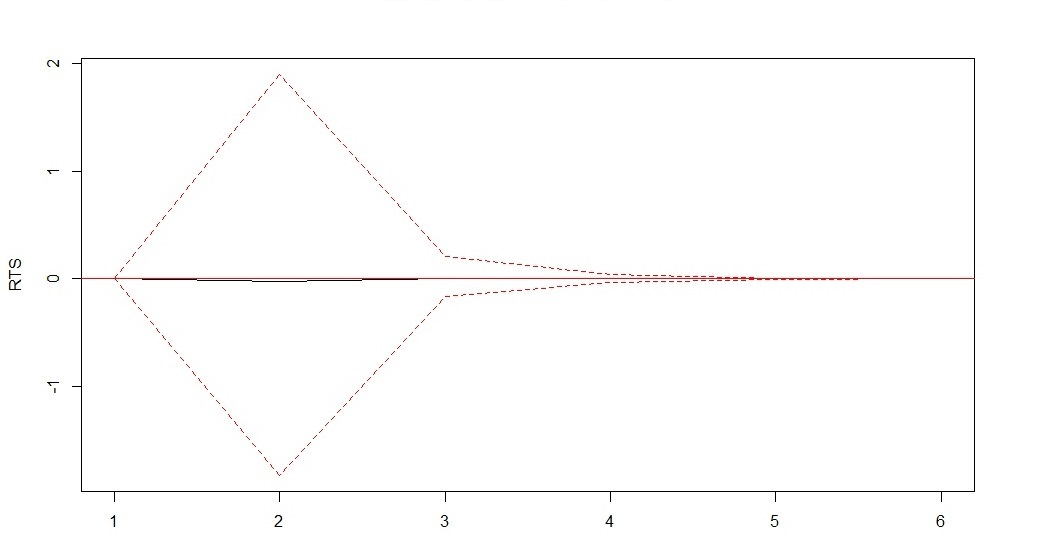
\includegraphics[width=1\linewidth]{1_rts_res}}
\end{minipage}
\vfill
\begin{minipage}[H]{0.49\linewidth}
\center{\footnotesize{Однодневная ставка МИАКР} \\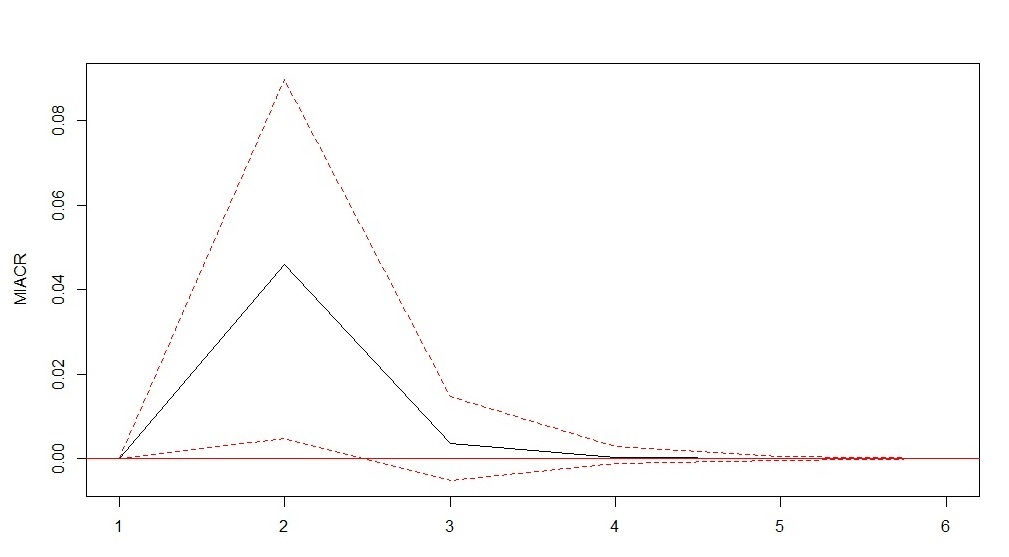
\includegraphics[width=1\linewidth]{1_miacr_res}} 
\end{minipage}
\caption{Функции импульсного отклика валютного курса, индекса РТС и ставки МИАКР на заявления Банка России}
\label{otkl_1}
\end{figure}

Из представленных графиков видно, что отклики валютного курса и индекса РТС на заявления Банка России незначимы. При этом, при ужесточающем заявлении, происходит шок в процентной ставке МИАКР. 

Такое поведение функций импульсного отклика может быть объяснено следующими особенностями монетарной политики Банка России:

\begin{Enumerate}

\item В конце 2014 года был произведен переход к политике плавающего валютного курса. В течение 2015 года объем валютных интервенций Банка России был сведен к минимуму. Большее внимание ЦБ стал уделять инфляции.

\item В декабре 2014 года Банк России поднял ключевую ставку до 17\%. В течение 2015 года ЦБ проводил умеренно-жёсткую монетарную политику. Интерес широких кругов общества был прикован к изменению ключевой ставки. В связи с этим заявления ЦБ за рассматриваемый период относились преимущественно к ставке процента. По отношению к действиям, связанным со ставкой ЦБ смог в течение рассматриваемого периода заработать себе репутацию.
\end{Enumerate} 

Дневная процентная ставка МИАКР реагирует на словесные интервенции ЦБ и в течение двух дней увеличивается на 0.04 базовых пункта. При этом в течение 4 дней происходит возврат ставки к прежнему уровню. Изменение ставки при наличии ужесточающего заявления со стороны ЦБ несущественно. Кроме того полученный результат является неустойчивым к способу построения доверительного интервала. При симуляции доверительного интервала с помощью метода Монте-Карло отклик получается незначимым. Однако стоит отметить, что бутсраповские доверительные интервалы считаются более достоверными.

В связи с тем, что в условиях инфляционного таргетирования валютный курс в России определяется внешними факторами, а именно динамикой цен на нефть, вполне целесообразным является включение в рассматриваемую модель стоимости нефти. 

\textbf{Вторая спецификация:}

\begin{equation}\label{f} 
\left\{
\begin{aligned}
&\Dt X_t = \a + \sum_{i=1}^p \a_{xi} \Dt X_{t-i} + \sum_{i=1}^p \a_{si} S_{t-i} + \sum_{i=1}^p \a_{oi} \Dt Oil_{t-i}+\a_d D_t +  u_{1t}, \\
&S_t = \b + \sum_{i=1}^p \b_{xi} \Dt X_{t-i} + \sum_{i=1}^p \b_{si} S_{t-i} + \sum_{i=1}^p \b_{0i} \Dt Oil_{t-i} + \b_d D_t +  u_{2t}, \\
&Oil_t =  Oil_{t-1} +  w_{3t}.
\end{aligned}
\right.
\end{equation}

Иначе говоря стоимость нефти является абсолютно экзогенной переменной и описывается с помощью случайного блуждания. На формирование её стоимости не влияют ни словесные интервенции, ни динамика валютного курса, на динамика процентной ставки, ни динамика индекса РТС. Таким образом уравнение~(\ref{f}) можно переписать в виде:  

\begin{equation}
\left\{
\begin{aligned}
&\Dt X_t = \a + \sum_{i=1}^p \a_{xi} \Dt X_{t-i} + \sum_{i=1}^p S_{t-i} + \sum_{i=0}^p \a_{oi} \Dt Oil_{t-i}+\a_d D_t +  \nu_{1t}, \\
&S_t = \b + \sum_{i=1}^p \b_{xi} \Dt X_{t-i} + \sum_{i=1}^p\b_{si} S_{t-i} + \sum_{i=0}^p \b_{0i} \Dt Oil_{t-i} + \a_d D_t +  \nu_{2t}.
\end{aligned}
\right.
\end{equation}

Рассмотрим модель с $p=1$. При построении функций импульсного отклика будем использовать упорядочивание $ \Dt Oil_t \to S_t \to \Dt X_t$.

Функции импульсного отклика валютного курса, индекса РТС и ставки МИАКР на заявления Банка России при такой спецификации и идентифицирующих предположениях будут иметь вид, представленный на рис.~\ref{otkl_2}. 

\begin{figure}[h]
\begin{minipage}[H]{0.49\linewidth}
\center{\footnotesize{Валютный курс} \\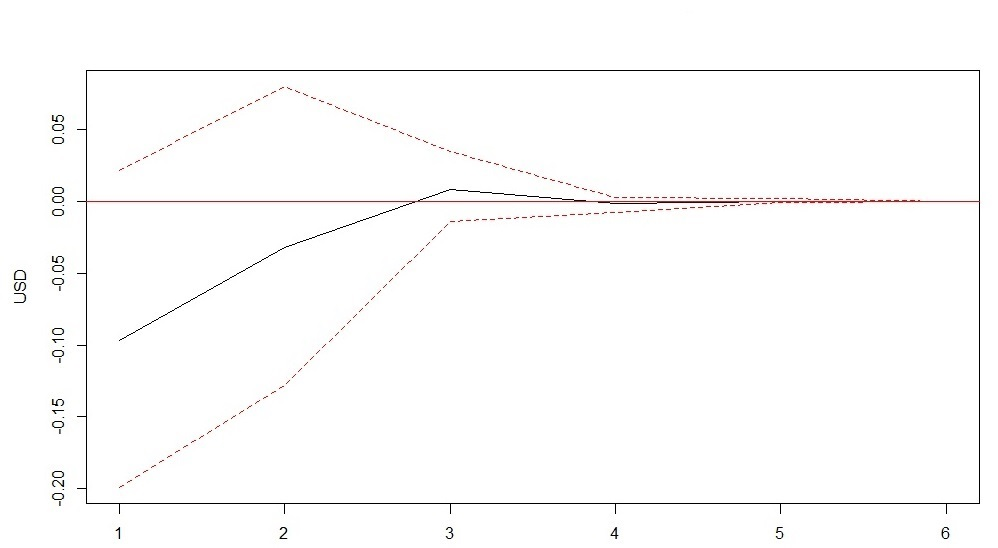
\includegraphics[width=1\linewidth]{2_usd_res}}
\end{minipage}
\hfill
\begin{minipage}[H]{0.49\linewidth}
\center{\footnotesize{Индекс РТС} \\ 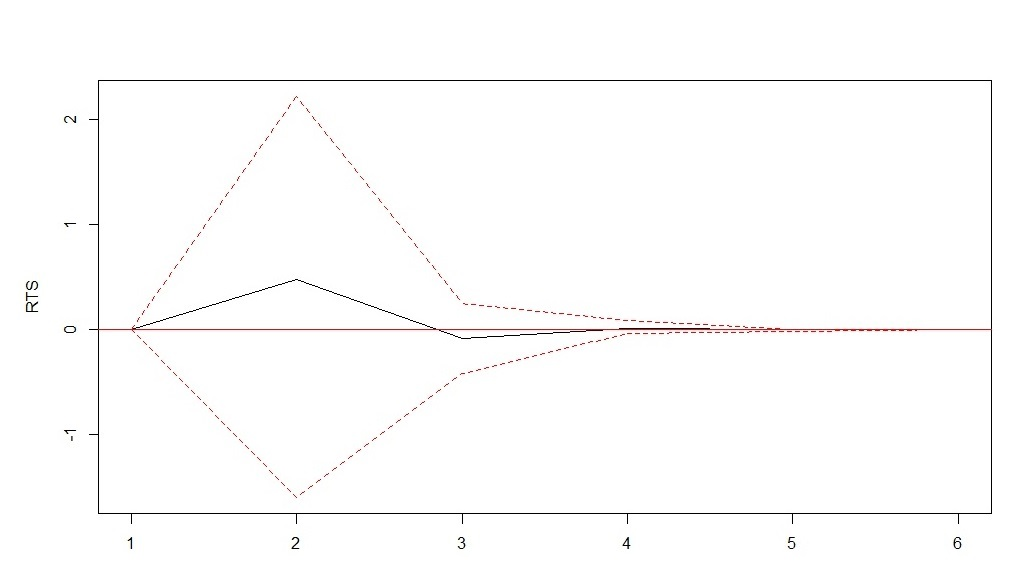
\includegraphics[width=1\linewidth]{2_rts_res}}
\end{minipage}
\vfill
\begin{minipage}[H]{0.49\linewidth}
\center{\footnotesize{Однодневная ставка МИАКР} \\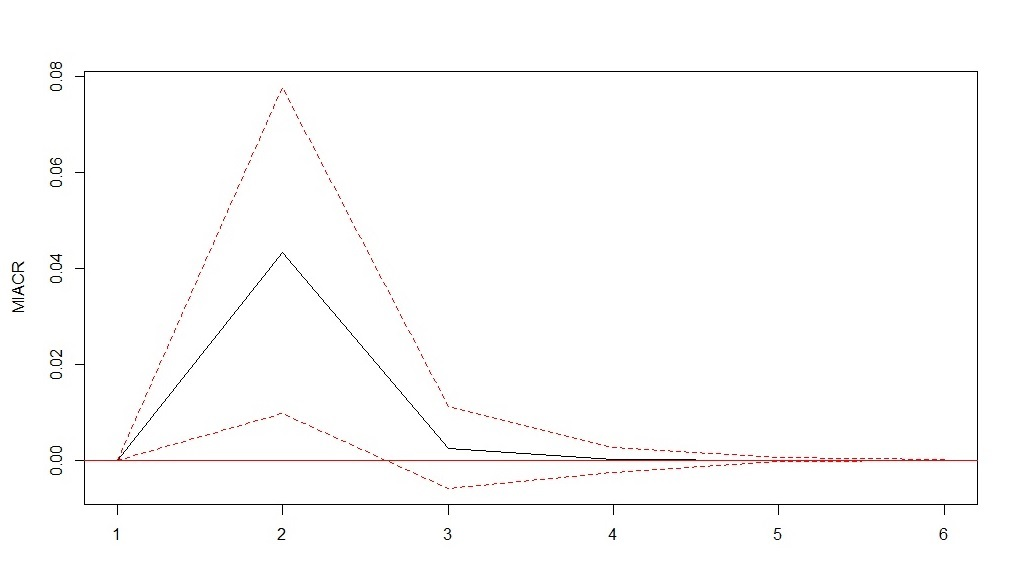
\includegraphics[width=1\linewidth]{2_miacr_res}} 
\end{minipage}
\caption{Функции импульсного отклика валютного курса, индекса РТС и ставки МИАКР на заявления Банка России}
\label{otkl_2}
\end{figure}
 
При словесной интервенции Банка России происходит прыжок однодневной ставки МИАКР в течение следующего дня после заявления. В течение четырёх дней ставка МИАКР возвращается к своему прежнему уровню. Вторая спецификация подтверждает выводы, полученные при первой спецификации модели. Импульсные отклики валютного курса и индекса РТС на словесные интервенции Банка России оказываются снова незначимыми.

Попробуем использовать некоторые другие подходы, описанные в обзоре эмпирических работ для решения прямой задачи.

\section{Решение прямой задачи с помощью подхода GARCH}

Для исследования динамики процентной ставки рассмотрим по аналогии с Эрманом и Фатшером~\cite{ehrmann2007communication} модель следующего вида 

\begin{equation}
\Dt MIACR_t = \beta_0 + \beta_1 S_t + D_t +\e_t.
\end{equation}

В рассматриваемой модели гипотеза о наличии ARCH-эффектов отвергается. Значимый вклад словесных интервенций в изменение ставок не наблюдается.

Для исследования динамики валютного курса рассмотрим по аналогии с Фатшером~\cite{fratzscher2008communication} модель вида

\begin{equation}
\Dt log(USD_t) = \beta_0 + \beta_1 S_t + \beta_2 VAL_t + \beta_3 ddd + \e_t.
\end{equation}

В рассматриваемой модели гипотеза о наличии ARCH-эффектов отвергается. Гипотеза о незначимости регрессии в целом не отвергается.

Таким образом словесные интервенции Банка России нельзя назвать эффективными в смысле, определенном ранее.

Попробуем с помощью теста Песарана-Тиммермана выяснить несёт ли ряд словесных интервенций информацию об изменении валютного курса, ставки МИАКР и индекса РТС.

\section{Тест Песарана-Тиммермана}

Тест Песарана-Тиммермана предназначен для проверки гипотезы $H_0:$ «Дискретный ряд $x_t$ не несёт информации об изменчивости дискретного ряда $y_t$»~\cite{pesaran2000recursive}.

Этот тест был подробно описан на странице~\pageref{P_T}. Попробуем применить его к имеющимся у нас данным.

Закодируем изменения переменных $USD$, $MIACR$, $RTS$ по шкале от -1 до 1. Рост переменной более чем на 0.2 пункта закодируем с помощью единицы. Падение переменной более чем на 0.2 пункта закодируем с помощью минус единицы. Изменение переменой на абсолютную величину, не превышающую 0.2 закодируем нулём. 

\begin{table}[h]
	\begin{center}
		\caption{Тест Песарана - Тиммермана}\label{P-Ttable}
		\begin{tabular}{|c|c|c|}
  		\hline
    	$y_t$ & $x_t$ & Наблюдаемое значение \\ \hline
  		$S_t$ & $USD_t$ & 0.33175  \\ \hline
  		$S_t$ & $MIACR_t$ & 0.24847  \\ \hline
  		$S_t$ & $RTS_t$ &  6.00676 \\ \hline
  		$S_t$ & $USD_{t-1}$ & 0.10386  \\ \hline
  		$S_t$ & $MIACR_{t-1}$ & 0.03446  \\ \hline
  		$S_t$ & $RTS_{t-1}$ & 1.13431  \\ \hline
  		$S_t$ & $USD_{t-2}$ & -0.19716  \\ \hline
  		$S_t$ & $MIACR_{t-2}$ & 0.00831  \\ \hline
  		$S_t$ & $RTS_{t-2}$ & 1.12777  \\ \hline
		\end{tabular}
	\end{center}
\end{table}

Тестирование будем проводить для текущего значения переменной, для первого лага и для второго лага. Код, используемый для проверки соответствующих гипотез приведен в приложении Г.

Результат расчёта наблюдаемых значений тестовой статистики представлен в таблице~\ref{P-Ttable}. Отметим, что в связи с отрицательным значением рассматриваемой статистики в случае $x_t = USD_{t-2}$ критерий Песарана-Тиммермана применить не удаётся. 

Предполагается, что переменные $x_t$ и $y_t$ принимают три различных дискретных значения. Тестовая статистика, при справедливости нулевой гипотезы, имеет асимптотическое $\chi^2_{4}$. Критическое значение для рассматриваемой статистики при 5\% уровне значимости составляет 9.48772. 

Таким образом гипотеза о том, что заявления Банка России не влияют на динамику каждого из рассматриваемых рядов, не отвергается.


%%% Оформляем Заключение и список литературы также как Оглавление и Введение

\titleformat{\chapter} 
    {\normalfont\bfseries\large}
    {\noindent}{0em}{\centering\normalfont\bfseries}  


\chapter*{Заключение}
\addcontentsline{toc}{chapter}{Заключение}

Начиная с 2014 г. Банк России, в связи с переходом к режиму инфляционного таргетирования, начал иначе перестраивать свою информационную политику, повышая уровень предсказуемости и прозрачности. Управление ожиданиями постепенно налаживается, однако в Центробанке отмечают, что уровень репутации, необходимый для эффективного использования информационного канала, ещё не достигнут. 

В данной работе были рассмотрены различные методы анализа влияния словесных интервенций на динамику различных макроэкономических переменных. С их помощью был проведён анализ информационной политики Банка России.  

В работе была сделана попытка ответить на два вопроса: «Оказывают ли в России словесные интервенции влияние на динамику валютного курса, индекса РТС и процентных ставок?» и «Можно ли по динамике валютного курса, индекса РТС или процентной ставки предсказать характер словесной интервенции?». 

В результате оценки порядковой пробит модели было получено, что нет никаких свидетельств статистической предсказуемости словесных интервенций. 

С помощью методологии VAR были построены функции импульсного отклика валютного курса, индекса РТС и ставки процента на словесные интервенции Банка России. Отклики индекса РТС и валютного курса оказались незначимы для всех рассмотренных спецификаций. Отклик однодневной процентной ставки на заявления Банка России МИАКР оказался значимым. При ужесточающем заявлении происходит рост ставки на 0.04 базовых пункта. Такое изменение процентной ставки является несущественным. Использование методологии GARCH и теста Песарана-Тимермана подтвердили, полученные с помощью методологии VAR результаты. В течение 2015 года словесные интервенции не оказывали влияния на динамику вышеперечисленных макроэкономических переменных. 

\newpage


%Если вашей душе мил bibtex и вы разберетесь как работать с пакетом bibtex-gost, то эта команда для вас!
%\printbibliography

%Команда для нормального названия у списка литры!
\renewcommand\bibname{Список литературы}

\begin{thebibliography}{99}
\addcontentsline{toc}{chapter}{Список литературы}%добавляем в соодержание

\bibitem{UDAEVA} Юдаева, К. В. О денежно-кредитной политике Банка России на современном этапе //Деньги и кредит. –- 2014. –- С. 13.

\bibitem{barro1986reputation} Barro, R. J. Reputation in a model of monetary policy with incomplete information //Journal of Monetary Economics. –- 1986. -- Т. 17. №. 1. С. 3-20.

\bibitem{barro1981positive} Barro, R. J., Gordon, D. B. A positive theory of monetary policy in a natural-rate model. –- 1981.

\bibitem{boivin2010has} Boivin J., Kiley M. T., Mishkin F. S. How has the monetary transmission mechanism evolved over time?. – National Bureau of Economic Research -- 2010.-– №. w15879.

\bibitem{cook1989effect} Cook T., Hahn T. The effect of changes in the federal funds rate target on market interest rates in the 1970s //Journal of Monetary Economics. –- 1989. –- Т. 24. №. 3. С. 331-351.


\bibitem{ehrmann2007communication} Ehrmann M., Fratzscher M. Communication by central bank committee members: Different strategies, same effectiveness? //Journal of Money, Credit and Banking. –- 2007. –- Т. 39. №. 2-3. С. 509-541.

\bibitem{fratzscher2008communication} Fratzscher M. Communication and exchange rate policy //Journal of Macroeconomics. -- 2008. -– Т. 30. №. 4. С. 1651-1672.

\bibitem{friedman1999future} Friedman B. M. The future of monetary policy: the central bank as an army with only a signal corps? //International finance. -– 1999. –- Т. 2. №. 3. С. 321-338.

\bibitem{gerlach2007interest} Gerlach S. et al. Interest rate setting by the ECB, 1999-2006: Words and deeds //International Journal of Central Banking. –- 2007. –- Т. 3. №. 3. С. 1-46.

\bibitem{guthrie2000open} Guthrie G., Wright J. Open mouth operations //Journal of Monetary Economics. –- 2000. -– Т. 46. №. 2. С. 489-516.

\bibitem{hayek1945use} Hayek F. A. The use of knowledge in society //The American economic review. –- 1945. -- С. 519-530.

\bibitem{kohn2003central} Kohn D. L. et al. Central bank talk: does it matter and why?//Divisions of Research \& Statistics and Monetary Affairs, Federal Reserve Board -- 2003.

\bibitem{kydland1977rules} Kydland F. E., Prescott E. C. Rules rather than discretion: The inconsistency of optimal plans //The journal of political Economy. –- 1977. –- С. 473-491.MLA	


\bibitem{melosi2013signaling} Melosi L. Signaling effects of monetary policy. –- 2013.

\bibitem{de2015brazilian} ГОСТ	
de Mendonça H. F., Faria I. Brazilian Central Bank communication and interest rate expectations //Macroeconomics and Finance in Emerging Market Economies. -– 2015. -- Т. 8. №. 1-2. С. 25-44.

\bibitem{mizen2009can} Mizen P. What can we learn from central bankers' words? Some nonparametric tests for the ECB //Economics Letters. –- 2009.-– Т. 103. №. 1. С. 29-32.

\bibitem{morris2005central} Morris S., Shin H. S. Central bank transparency and the signal value of prices //Brookings Papers on Economic Activity. -– 2005. -– Т. 2005. №. 2. С. 1-66.

\bibitem{palmqvist1998central} Palmqvist S. Why Central Banks Announce their Objectives: Monetary Policy with Discretionary Signalling. -- 1998.

\bibitem{pesaran2000recursive} Pesaran M. H., Timmermann A. A recursive modelling approach to predicting UK stock returns //The Economic Journal. –- 2000. -– Т. 110. №. 460. С. 159-191.

\bibitem{phillips1958relation} Phillips A. W. The Relation between unemployment and the rate of change of money wage rates in the United Kingdom, 1861–19571 //economica. -– 1958. –- Т. 25. №. 100. С. 283-299.

\bibitem{svensson2000should} Svensson L. E. O. How should monetary policy be conducted in an era of price stability?. – National bureau of economic research -- 2000. -– №. w7516.

\bibitem{takagi2013central} Takagi S. et al. Central Bank Independence and the Signaling Effect of Intervention: A Preliminary Exploration. –- 2013. -– №. 13-04.

\bibitem{thornton2004fed} Thornton D. L. The Fed and short-term rates: Is it open market operations, open mouth operations or interest rate smoothing? //Journal of Banking \& Finance. –-- 2004. -- Т. 28. №. 3. С. 475-498.

\bibitem{woodford2005central} Woodford M. Central bank communication and policy effectiveness. //National Bureau of Economic Research -- b2005. -– №. w11898.

\end{thebibliography}



%%%%%%%%%%%%%%%%%%%% Приложения %%%%%%%%%%%%%%%%%%%%

\newpage

\appendix
\renewcommand{\thechapter}{\Asbuk{chapter}}

%tocloft
\addtocontents{toc}{
\protect\renewcommand
\protect\cftchappresnum{Приложение~}
\protect\renewcommand
\protect\cftchapnumwidth{8.6 em}
}

%titlesec
\titleformat{\chapter}
 {\normalfont\bfseries\large}{\chaptertitlename~\thechapter.}{1 em}{\normalfont}

\titleformat{\section}{\bfseries}{\thesection}{1em}{}


\chapter[Программа~~  для~~ поиска~~ и~~ выгрузки~~   статей, касающихся Банка России из архива газеты Ведомости]{Программа для поиска и выгрузки статей, касающихся Банка Росии из архива газеты Ведомости (Python)}\label{app-a}

\begin{minted}[breaklines]{python}
import requests
import re
from bs4 import BeautifulSoup
import pandas as pd
import numpy as np
import pickle

#Вспомогательная функция для получения правильного количества дней. Работает даже с високосным годом.
def monthlength(month,year):
    if year % 4 == 0:
         VisYear = 29
    else:
         VisYear = 28
    return [31,VisYear,31,30,31,30,31,31,30,31,30,31][month]

#Загрузка кода страницы по дню, месяцу и году.
mainpage = "http://www.vedomosti.ru/archive/"
def getPageCode(year,month,day):
    # выгружает данные по ссылке
    response = requests.get(mainpage+str(year)+"/"+str(month)+"/"+str(day))                                      
    # переводит их в читаемый формат, который можно вывести на экран    
    html = response.content           
    # отсекает кучу всяких ненужных вещей и запускает поиск по тегам в html     
    soup = BeautifulSoup(html,"lxml")   
    # отсекает ошибки, когда в 1 на 10000 статей не читается какой-то символ!
    soup = soup.encode("utf-8")       
    return soup       

#Функция, возвращающая список ссылок за конкретное число.
def getListRefs(year,month,day):
    s = str(getPageCode(year,month,day))
    ss = re.split('<div class="b-article__title">',s)[1:]
    w = [re.split('href=\"|\">',item)[1] for item in ss]
    return w

#Функция, возвращающая заголовок статьи и её текст
def TitleText(url):
    response = requests.get("http://www.vedomosti.ru"+url)
    html = response.content
    soup = BeautifulSoup(html,"html.parser")
    tit = str(soup)
    tit = re.split('<h1|</h1',tit)[1]
    texts = soup.findAll(text=True)
    texts = str(texts)
    text = re.split("Справочник компаний|Выбор редактора|Выбор читателей|Комментарии",texts)[1]
    text = BeautifulSoup(text,"html.parser")
    tit = BeautifulSoup(tit,"html.parser")
    [s.extract() for s in text(['style', 'script','[document]', 'head', 'title'])]
    [s.extract() for s in tit(['style', 'script','[document]', 'head', 'title'])]
    visible_text = str(text.getText())
    visible_title = str(tit.getText())    
    visible_title = re.sub(u"[^а-яА-Я.,\-\s]", "",visible_title) #очистка заголовка от хлама!
    visible_title = re.sub(u"[.,\-\s]{3,}", " ",visible_title).lower()    
    visible_text = re.sub(u"[^а-яА-Я.,\-\s]", "",visible_text)   
    visible_text = re.sub(u"[.,\-\s]{3,}", " ",visible_text).lower() #очистка текста от хлама!  
    dict = {"text": visible_text,"title": visible_title,"url":url}
    return dict

#Новость считается относящейся к ЦБ, если в заголовке фигурирует одно из слов: Набиулл, Центробанк, Юдаев, Банк России, ЦБ.
def isCBNews(url):
    df = TitleText(url)
    df_title = df['title'].lower()
    df_text = df['text'].lower()
    if df_title.count(" цб ")+df_title.count(" набиулл")    +df_title.count(" центробанк")+ df_title.count(" юдаев")    +df_title.count(" банк россии ")>0:
        answer = [1,df]
    else:
        answer = [0,0]
    return(answer)

#Функция, которая выдает все ссылки о ЦБ в конкретный день, текст статьи.
def getCBList(year,month,day):
    zerone = [isCBNews(item)[1] for item in 
    getListRefs(year,month,day) if isCBNews(item)[0]==1]
    return(zerone)
\end{minted}

Итак, мы можем достать с помощью функции getCBList матрицу для каждой даты, каждая строка которой будет иметь вид: [ссылка,найдена ли статья по заголовку, был ли у статьи приоритет, текст].

Цикл, который выгрузит все новости о ЦБ за Январь в кучу маленьких файлов на жесткий диск будет иметь вид:

\begin{minted}[breaklines]{python}
def DaysOfYear(year):
    def Days(month):
        return([i for i in range(1,monthlength(month,2015)+1)])
    s = []
    for i in range(0,12):
        s.append(Days(i))
    return(s)
    
cd "C:\Users\zero\Desktop\mydata"

lll = DaysOfYear(2015)[0]
for number in lll:
    pickle.dump(getCBList(2015,1,number), 
    open(str(number)+'.txt', "wb" )) 
\end{minted}

Остальные месяцы выгружаются аналогичным образом. Теперь необходимо каждую из новостей, имеющих отношение к ЦБ дать оценку. Какой именно характер имеет словесная интервенция, отраженная в данной новости. Если она ведет к ужесточению политики, будем присваивать 1, если к смягчению, то -1. В итоге на выходе будем получать матрицу, каждая строка которой имеет вид [дата, смягчение или ужесточение].



\chapter[Программа~~  для~~  оценки~~  порядковой \\ пробит модели (язык R)]{Программа для оценки порядковой пробит модели (язык R)}\label{app-b}


\begin{minted}[breaklines]{R}
library("dplyr")
library("erer")
library("vcd")
library("ggplot2")
library("reshape2")
library("AUC")
library("forecast")
library("zoo") 
library("vars")
library("ordinal")

options(stringsAsFactors=FALSE)

ALLdata <- read.csv("data.txt",sep="\t",dec=".",header=TRUE)
data_usd <- data.frame(ALLdata$STATEMENT[-1],diff(ALLdata$USD,1))
data_rts <- data.frame(ALLdata$STATEMENT[-1],diff(ALLdata$RTS,1))
data_miacr <- data.frame(ALLdata$STATEMENT[-1],diff(ALLdata$MIACR,1))

#Подготовительная работа!
#Функция, создающая dataframe с запаздываниями
change_data <- function(data){
names(data) <-c("V1","V2")
tf <- zoo(data)
usd_lags1 <- lag(tf$V1,-1*0:10,na.pad=TRUE)
usd_lags2 <- lag(tf$V2,-1*0:10,na.pad=TRUE)
df <- data.frame(usd_lags1,usd_lags2)
names(df) <- c(paste0('Y', 0:10), paste0('V', 0:10))
df <- mutate(df,Y0=as.factor(Y0),Y1=as.factor(Y1),Y2=as.factor(Y2),          Y3=as.factor(Y3),Y4=as.factor(Y4),Y5=as.factor(Y5),          Y6=as.factor(Y6),Y7=as.factor(Y7),Y8=as.factor(Y8),		  Y9=as.factor(Y9),Y10=as.factor(Y10))
return(df)
}

#функция, выбирающая для конкретного dataframe оптимальное по 
#критерию шварца количество лагов
minbic <- function(dddf){
df = change_data(dddf)

#Нам нужно перебрать все возможные сочетания лагов. Сделаем это.
dep_var <- 'Y0'
indep_vars <- setdiff(names(df), dep_var)
iv_1 <- indep_vars[1:10]
iv_2 <- indep_vars[11:20]

#Определим оптимальное количество запаздываний:
order <- c()
min <- 10^10
for(i in 1:10){
  for(j in 1:10){
    reg <- paste(c("Y0",paste(c(paste(iv_1[1:j],collapse="+"),    paste(iv_2[1:i],collapse="+")),collapse="+")),collapse="~")
    fm <- glm(data = df,reg)
    if(BIC(fm)<min){
      min <- BIC(fm)
      order <- c(j,i)
    }
  }
}
return(order)
}

minbic(data_usd)
minbic(data_miacr)
minbic(data_rts)
\end{minted}



\newpage
Выпускная квалификационная работа выполнена мной совершенно самостоятельно. Все использованные в работе материалы и концепции из опубликованной научной литературы и других источников имеют ссылки на них.

\vspace{2ex}

\noindent Объем работы  \rule{3em}{0.5pt} листа(ов).

\vspace{2ex}

\noindent Объем приложений \rule{3em}{0.5pt} листа(ов).

\vspace{4ex}

\noindent <<\rule{2em}{0.5pt}>> \rule{5em}{0.5pt} 201\rule{1em}{0.5pt} г. 

\vspace{4ex}

\noindent \rule{10em}{0.5pt} Ульянкин Филипп Валерьевич


\end{document}